% Capitolul 4: Cointegrare: VECM, ARDL și date panel
% Analiza avansată a seriilor de timp și previziune -- Programul de master Statistică aplicată și data science, anul I, semestrul 2, Academia de Studii Economice din București
% GENERAT de latex/build_chapter4.py -- modificați generatorul, nu acest fișier.

\newcommand{\coursename}{Analiza avansată a seriilor de timp și previziune}
\def\atslang{ro}
% Preambul comun ATS -- Analiza avansată a seriilor de timp și previziune / Advanced Time Series Analysis and Forecasting
% (Beamer, 16:9). Același design ca MFM, SFM și TSA (copiat din TSA, 5 octombrie 2026). Înainte de % Preambul comun ATS -- Analiza avansată a seriilor de timp și previziune / Advanced Time Series Analysis and Forecasting
% (Beamer, 16:9). Același design ca MFM, SFM și TSA (copiat din TSA, 5 octombrie 2026). Înainte de % Preambul comun ATS -- Analiza avansată a seriilor de timp și previziune / Advanced Time Series Analysis and Forecasting
% (Beamer, 16:9). Același design ca MFM, SFM și TSA (copiat din TSA, 5 octombrie 2026). Înainte de \input{../../latex/preamble} se definește
%   \newcommand{\coursename}{Advanced Time Series Analysis and Forecasting}          (EN)
%   \newcommand{\coursename}{Analiza avansată a seriilor de timp și previziune}       (RO)  și  \def\atslang{ro}
% Fișierele .tex se află în EN/Courses, EN/Seminars, RO/Cursuri, RO/Seminarii (două niveluri sub rădăcină).
% Deck-urile sînt generate de latex/build_chapterN.py / build_seminarN.py (vezi latex/ats_build.py).

\documentclass[9pt, aspectratio=169, t]{beamer}
\providecommand{\coursename}{Advanced Time Series Analysis and Forecasting}

% Ensure content fits on slides
\setbeamersize{text margin left=8mm, text margin right=8mm}
% Smaller institute font (title page)
\setbeamerfont{institute}{size=\footnotesize}

%=============================================================================
% THEME AND STYLE CONFIGURATION
%=============================================================================
\usetheme{default}
% Using default theme for clean header/footer control

% Color Palette (matching Redispatch PDF)
\definecolor{MainBlue}{RGB}{26, 58, 110}
\definecolor{AccentBlue}{RGB}{26, 58, 110}
\definecolor{IDAred}{RGB}{205, 0, 0}
\definecolor{DarkGray}{RGB}{51, 51, 51}
\definecolor{MediumGray}{RGB}{128, 128, 128}
\definecolor{LightGray}{RGB}{248, 248, 248}
\definecolor{VeryLightGray}{RGB}{235, 235, 235}
\definecolor{KeynoteGray}{RGB}{218, 218, 218}
\definecolor{SectionGray}{RGB}{120, 120, 120}
\definecolor{FooterGray}{RGB}{100, 100, 100}
\definecolor{Crimson}{RGB}{220, 53, 69}
\definecolor{Forest}{RGB}{46, 125, 50}
\definecolor{Amber}{RGB}{181, 133, 63}
\definecolor{Orange}{RGB}{230, 126, 34}
\definecolor{Purple}{RGB}{142, 68, 173}

% Gradient background (exact Keynote 315° gradient: white to RGB 218,218,218)
\setbeamertemplate{background}{%
    \begin{tikzpicture}[remember picture, overlay]
        \shade[shading=axis, shading angle=315,
        top color=white, bottom color=KeynoteGray]
        (current page.south west) rectangle (current page.north east);
    \end{tikzpicture}%
}
% Fallback solid color for compatibility
\setbeamercolor{background canvas}{bg=}

\setbeamercolor{palette primary}{bg=MainBlue, fg=white}
\setbeamercolor{palette secondary}{bg=MainBlue!85, fg=white}
\setbeamercolor{palette tertiary}{bg=MainBlue!70, fg=white}
\setbeamercolor{structure}{fg=MainBlue}
\setbeamercolor{title}{fg=IDAred}
\setbeamercolor{frametitle}{fg=IDAred, bg=}
\setbeamercolor{block title}{bg=MainBlue, fg=white}
\setbeamercolor{block body}{bg=VeryLightGray, fg=DarkGray}
\setbeamercolor{block title alerted}{bg=Crimson, fg=white}
\setbeamercolor{block body alerted}{bg=Crimson!8, fg=DarkGray}
\setbeamercolor{block title example}{bg=Forest, fg=white}
\setbeamercolor{block body example}{bg=Forest!8, fg=DarkGray}
\setbeamercolor{item}{fg=MainBlue}

% Footer colors (override Madrid theme blue)
\setbeamercolor{author in head/foot}{fg=FooterGray, bg=}
\setbeamercolor{title in head/foot}{fg=FooterGray, bg=}
\setbeamercolor{date in head/foot}{fg=FooterGray, bg=}
\setbeamercolor{section in head/foot}{fg=FooterGray, bg=}
\setbeamercolor{subsection in head/foot}{fg=FooterGray, bg=}

% Bullet styles (apply everywhere including blocks)
\setbeamertemplate{itemize item}{\color{MainBlue}$\boxdot$}
\setbeamertemplate{itemize subitem}{\color{MainBlue}$\blacktriangleright$}
\setbeamertemplate{itemize subsubitem}{\color{MainBlue}\tiny$\bullet$}
\setbeamertemplate{itemize/enumerate body begin}{\normalsize}
\setbeamertemplate{itemize/enumerate subbody begin}{\normalsize}

% Item spacing - compact style
\setlength{\leftmargini}{10pt}       % Level 1: minimal indent
\setlength{\leftmarginii}{10pt}      % Level 2: minimal additional indent
% Compact list spacing (zero extra space before/after lists in blocks)
\makeatletter
\def\@listi{\leftmargin\leftmargini \topsep 0pt \parsep 0pt \itemsep 0pt}
\def\@listii{\leftmargin\leftmarginii \topsep 0pt \parsep 0pt \itemsep 0pt}
\makeatother

\setbeamertemplate{navigation symbols}{}

%=============================================================================
% CUSTOM HEADLINE
%=============================================================================
\setbeamertemplate{headline}{%
    \vskip10pt%
    \hbox to \paperwidth{%
        \hskip0.5cm%
        {\small\color{FooterGray}\renewcommand{\hyperlink}[2]{##2}\insertsectionhead}%
        \hfill%
        \textcolor{FooterGray}{\small\insertframenumber}%
        \hskip0.5cm%
    }%
    \vskip4pt%
    {\color{FooterGray}\hrule height 0.4pt}%
}

%=============================================================================
% CUSTOM FOOTER
%=============================================================================
\usepackage{fontawesome5}

\setbeamertemplate{footline}{%
    {\color{FooterGray}\hrule height 0.4pt}%
    \vskip4pt%
    \hbox to \paperwidth{%
        \hskip0.5cm%
        \textcolor{FooterGray}{\small\coursename}%
        \hfill%
        \raisebox{-0.1em}{%
            \begin{tikzpicture}[x=0.08em, y=0.08em, line width=0.4pt]
                \draw[FooterGray] (0,3) -- (1,4) -- (2,3.5) -- (3,5) -- (4,4) -- (5,6) -- (6,5.5) -- (7,4) -- (8,5) -- (9,7) -- (10,6) -- (11,5) -- (12,6.5) -- (13,8) -- (14,7) -- (15,6) -- (16,7.5) -- (17,9) -- (18,8) -- (19,7) -- (20,8.5) -- (21,10) -- (22,9) -- (23,8) -- (24,9.5);
            \end{tikzpicture}%
        }%
        \hskip0.5cm%
    }%
    \vskip6pt%
}

%=============================================================================
% PACKAGES
%=============================================================================
\usepackage[utf8]{inputenc}
\DeclareUnicodeCharacter{03B1}{\ensuremath{\alpha}}
\usepackage[T1]{fontenc}
\usepackage{amsmath, amssymb, amsthm}
\usepackage{mathtools}
\usepackage{bm}
\usepackage{tikz}
\usetikzlibrary{arrows.meta, positioning, shapes, calc, decorations.pathreplacing, shadings}
\usepackage{booktabs}
\usepackage{multirow}
\usepackage{array}
\usepackage{graphicx}
\usepackage{animate}
\usepackage{hyperref}
\usepackage{colortbl}
\usepackage{listings}
\lstset{language=Python, basicstyle=\ttfamily\scriptsize, keywordstyle=\color{MainBlue}\bfseries,
  commentstyle=\color{Forest}, stringstyle=\color{Crimson}, breaklines=true,
  frame=none, backgroundcolor=\color{VeryLightGray}, xleftmargin=2mm}
\hypersetup{colorlinks=true, linkcolor=MainBlue, urlcolor=MainBlue}
\graphicspath{{../../logos/}{../../charts/}{../../photos/}}
\usepackage{xcolor}
\hfuzz=2pt  % Suppress tiny overfull warnings (<2pt)
\vfuzz=2pt  % Suppress tiny vertical overfull warnings (<2pt)

%=============================================================================
% QUANTLET COMMANDS
%   \quantlet{<displayed name>}{<url>}       (generic)
%   \atsquantlet{Ch_05}{ATS_ch5_garch}       -> https://github.com/danpele/Advanced-Time-Series/tree/main/Quantlets/Ch_05/ATS_ch5_garch
%   \qlurl{<folder>} is defined per chapter by the generator (Quantlets/Ch_NN/<folder>)
%=============================================================================
\newcommand{\atsrepo}{https://github.com/danpele/Advanced-Time-Series}
\newcommand{\atsqlbase}{https://github.com/danpele/Advanced-Time-Series/tree/main/Quantlets}
\newcommand{\quantlet}[2]{%
    \hfill\href{#2}{%
        \raisebox{-0.15em}{
\includegraphics[height=0.7em]{ql_logo.png}}%
        \textcolor{MainBlue}{\tiny\ #1}%
    }%
}
\newcommand{\atsquantlet}[2]{\quantlet{\detokenize{#2}}{\atsqlbase/#1/#2}}

%=============================================================================
% NOTEBOOKS (Google Colab)
%   \colaburl{notebooks/EN/chapter5_seminar_notebook.ipynb} -> the Colab link of a file in the ATS repo
%   \nb: the chapter notebook (each seminar deck redefines it with \renewcommand)
%=============================================================================
\newcommand{\colaburl}[1]{https://colab.research.google.com/github/danpele/Advanced-Time-Series/blob/main/#1}
\newcommand{\nb}{https://colab.research.google.com/github/danpele/Advanced-Time-Series/tree/main/notebooks/EN}
\newcommand{\nbname}{notebooks/EN}

%=============================================================================
% SLIDE HELPERS (used by the generators; the same as in MFM)
%=============================================================================
% local font size for list bodies (the preamble forces \normalsize)
\newcommand{\itemsize}[1]{\setbeamertemplate{itemize/enumerate body begin}{#1}\setbeamertemplate{itemize/enumerate subbody begin}{#1}}
\newcommand{\intitle}[1]{{\hypersetup{urlcolor=white}#1}}   % white links inside coloured title bars
\newcommand{\imgcap}[1]{{\scriptsize #1}\\[0.5mm]}          % caption under a photo
\newcommand{\imgcredit}[2]{{\tiny\color{FooterGray}\href{#1}{#2}}}   % image credit: source URL, author/licence
\newcommand{\aiprompt}[1]{{\ttfamily\color{MainBlue}#1}}     % a prompt to an AI assistant

%=============================================================================
% SEMINARS: student version by default; the instructor wrapper *_solutions.tex sets \solutionstrue
%=============================================================================
\makeatletter\@ifundefined{ifsolutions}{\expandafter\newif\csname ifsolutions\endcsname}{}\makeatother
\newcommand{\solonly}[1]{\ifsolutions #1\fi}
\newcommand{\propsub}{\ifsolutions\else\framesubtitle{\ifdefined\atslang Rezolvarea se discută la seminar\else Solution discussed in class\fi}\fi}

%=============================================================================
% APPENDIX AND CHAPTER LINKS (latex/appendix_links.py writes the calls; it also re-declares these
% macros before \begin{document}, so the decks compile with or without this preamble block)
%=============================================================================
\providecommand{\atsapplink}[3]{\hypertarget{#2}{}\hyperlink{#1}{\beamergotobutton{#3}}}
\providecommand{\atsappback}[2]{\begin{tikzpicture}[remember picture,overlay]\node[anchor=south east] at ([xshift=-3mm,yshift=7mm]current page.south east){\hyperlink{#1}{\beamerreturnbutton{#2}}};\end{tikzpicture}}
\providecommand{\atschlink}[2]{\href{#1}{#2}}
\providecommand{\atschlinkt}[2]{\href{#1}{\usebeamercolor[fg]{frametitle}#2}}

%=============================================================================
% QUANTINAR COMMAND: link către un curs Quantinar (subiecte avansate)
%=============================================================================
\newcommand{\quantinar}[2]{%
    \href{#2}{%
        \raisebox{-0.15em}{
\includegraphics[height=0.8em]{qr_logo.png}}%
        \textcolor{MainBlue}{\scriptsize\ #1}%
    }%
}

%=============================================================================
% CUSTOM TITLE PAGE
%=============================================================================
\defbeamertemplate*{title page}{hybrid}[1][]
{
    \vspace{0.2cm}
    % Logos row - top header (with clickable links)
    \begin{center}
        \href{https://www.ase.ro}{
\includegraphics[height=1.0cm]{ase_logo.png}}\hspace{0.3cm}%
        \href{https://theida.net}{
\includegraphics[height=1.0cm]{ida_logo.png}}\hspace{0.3cm}%
        \href{https://blockchain-research-center.com}{
\includegraphics[height=1.0cm]{brc_logo.png}}\hspace{0.3cm}%
        \href{https://www.ai4efin.ase.ro}{
\includegraphics[height=1.0cm]{ai4efin_logo.png}}\hspace{0.3cm}%
        \href{https://ipe.ro/new}{
\includegraphics[height=1.0cm]{acad_logo.png}}\hspace{0.3cm}%
        \href{https://www.digital-finance-msca.com}{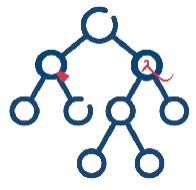
\includegraphics[height=1.0cm]{msca_logo.png}}%
    \end{center}

    \vspace{0.6cm}

    % Main title with Q logos on sides (with clickable links)
    \begin{center}
        \begin{minipage}{0.1\textwidth}
            \centering
            \href{https://quantlet.com}{
\includegraphics[height=1.1cm]{ql_logo.png}}
        \end{minipage}%
        \begin{minipage}{0.78\textwidth}
            \centering
            {\LARGE\bfseries\usebeamercolor[fg]{title}\inserttitle}

            \vspace{0.3cm}

            {\usebeamerfont{subtitle}\usebeamercolor[fg]{title}\insertsubtitle}
        \end{minipage}%
        \begin{minipage}{0.1\textwidth}
            \centering
            \href{https://quantinar.com}{
\includegraphics[height=1.1cm]{qr_logo.png}}
        \end{minipage}
    \end{center}

    \vspace{0.6cm}

    % Authors (left aligned)
    \hspace{0.5cm}{\usebeamerfont{author}\insertauthor}

    \vspace{0.3cm}

    % Institute/Affiliations (left aligned)
    \hspace{0.5cm}\begin{minipage}[t]{0.9\textwidth}
        \raggedright\small\insertinstitute
    \end{minipage}
}

%=============================================================================
% THEOREM ENVIRONMENTS
%=============================================================================
\theoremstyle{definition}
\setbeamertemplate{theorems}[numbered]
\ifdefined\atslang
\newtheorem{defn}{Definiție}
\newtheorem{thm}{Teoremă}
\newtheorem{prop}{Propoziție}
\newtheorem{rmk}{Observație}
\else
\newtheorem{defn}{Definition}
\newtheorem{thm}{Theorem}
\newtheorem{prop}{Proposition}
\newtheorem{rmk}{Remark}
\fi

%=============================================================================
% CENTRED MINIPAGE (no extra vertical space)
%=============================================================================
\newenvironment{cminipage}[1]{%
    \par\noindent\hfill\begin{minipage}{#1}\ignorespaces
}{%
    \end{minipage}\hfill\null\par
}

%=============================================================================
% CUSTOM COMMANDS
%=============================================================================
\newcommand{\E}{\mathbb{E}}
\newcommand{\Var}{\text{Var}}
\newcommand{\Cov}{\text{Cov}}
\newcommand{\Corr}{\text{Corr}}
\newcommand{\R}{\mathbb{R}}
\newcommand{\N}{\mathbb{N}}
\newcommand{\Z}{\mathbb{Z}}
\newcommand{\B}{\mathbf{B}}
\newcommand{\imark}{\textcolor{MainBlue}{\textbullet}}
\newcommand{\RMSE}{\text{RMSE}}
\newcommand{\MAE}{\text{MAE}}
\newcommand{\MAPE}{\text{MAPE}}

% Boldface vector/matrix commands (VAR, VECM, state space)
\newcommand{\bY}{\mathbf{Y}}
\newcommand{\bX}{\mathbf{X}}
\newcommand{\bA}{\mathbf{A}}
\newcommand{\bB}{\mathbf{B}}
\newcommand{\bepsilon}{\boldsymbol{\varepsilon}}
\newcommand{\bSigma}{\boldsymbol{\Sigma}}
\newcommand{\bPhi}{\boldsymbol{\Phi}}
\newcommand{\bGamma}{\boldsymbol{\Gamma}}
\newcommand{\bPi}{\boldsymbol{\Pi}}
\newcommand{\bc}{\mathbf{c}}
\newcommand{\balpha}{\boldsymbol{\alpha}}
\newcommand{\bbeta}{\boldsymbol{\beta}}
\newcommand{\bvarepsilon}{\boldsymbol{\varepsilon}}

% Seminar marks
\newcommand{\correct}{\textcolor{Forest}{\checkmark}}
\newcommand{\incorrect}{\textcolor{Crimson}{\texttimes}}
 se definește
%   \newcommand{\coursename}{Advanced Time Series Analysis and Forecasting}          (EN)
%   \newcommand{\coursename}{Analiza avansată a seriilor de timp și previziune}       (RO)  și  \def\atslang{ro}
% Fișierele .tex se află în EN/Courses, EN/Seminars, RO/Cursuri, RO/Seminarii (două niveluri sub rădăcină).
% Deck-urile sînt generate de latex/build_chapterN.py / build_seminarN.py (vezi latex/ats_build.py).

\documentclass[9pt, aspectratio=169, t]{beamer}
\providecommand{\coursename}{Advanced Time Series Analysis and Forecasting}

% Ensure content fits on slides
\setbeamersize{text margin left=8mm, text margin right=8mm}
% Smaller institute font (title page)
\setbeamerfont{institute}{size=\footnotesize}

%=============================================================================
% THEME AND STYLE CONFIGURATION
%=============================================================================
\usetheme{default}
% Using default theme for clean header/footer control

% Color Palette (matching Redispatch PDF)
\definecolor{MainBlue}{RGB}{26, 58, 110}
\definecolor{AccentBlue}{RGB}{26, 58, 110}
\definecolor{IDAred}{RGB}{205, 0, 0}
\definecolor{DarkGray}{RGB}{51, 51, 51}
\definecolor{MediumGray}{RGB}{128, 128, 128}
\definecolor{LightGray}{RGB}{248, 248, 248}
\definecolor{VeryLightGray}{RGB}{235, 235, 235}
\definecolor{KeynoteGray}{RGB}{218, 218, 218}
\definecolor{SectionGray}{RGB}{120, 120, 120}
\definecolor{FooterGray}{RGB}{100, 100, 100}
\definecolor{Crimson}{RGB}{220, 53, 69}
\definecolor{Forest}{RGB}{46, 125, 50}
\definecolor{Amber}{RGB}{181, 133, 63}
\definecolor{Orange}{RGB}{230, 126, 34}
\definecolor{Purple}{RGB}{142, 68, 173}

% Gradient background (exact Keynote 315° gradient: white to RGB 218,218,218)
\setbeamertemplate{background}{%
    \begin{tikzpicture}[remember picture, overlay]
        \shade[shading=axis, shading angle=315,
        top color=white, bottom color=KeynoteGray]
        (current page.south west) rectangle (current page.north east);
    \end{tikzpicture}%
}
% Fallback solid color for compatibility
\setbeamercolor{background canvas}{bg=}

\setbeamercolor{palette primary}{bg=MainBlue, fg=white}
\setbeamercolor{palette secondary}{bg=MainBlue!85, fg=white}
\setbeamercolor{palette tertiary}{bg=MainBlue!70, fg=white}
\setbeamercolor{structure}{fg=MainBlue}
\setbeamercolor{title}{fg=IDAred}
\setbeamercolor{frametitle}{fg=IDAred, bg=}
\setbeamercolor{block title}{bg=MainBlue, fg=white}
\setbeamercolor{block body}{bg=VeryLightGray, fg=DarkGray}
\setbeamercolor{block title alerted}{bg=Crimson, fg=white}
\setbeamercolor{block body alerted}{bg=Crimson!8, fg=DarkGray}
\setbeamercolor{block title example}{bg=Forest, fg=white}
\setbeamercolor{block body example}{bg=Forest!8, fg=DarkGray}
\setbeamercolor{item}{fg=MainBlue}

% Footer colors (override Madrid theme blue)
\setbeamercolor{author in head/foot}{fg=FooterGray, bg=}
\setbeamercolor{title in head/foot}{fg=FooterGray, bg=}
\setbeamercolor{date in head/foot}{fg=FooterGray, bg=}
\setbeamercolor{section in head/foot}{fg=FooterGray, bg=}
\setbeamercolor{subsection in head/foot}{fg=FooterGray, bg=}

% Bullet styles (apply everywhere including blocks)
\setbeamertemplate{itemize item}{\color{MainBlue}$\boxdot$}
\setbeamertemplate{itemize subitem}{\color{MainBlue}$\blacktriangleright$}
\setbeamertemplate{itemize subsubitem}{\color{MainBlue}\tiny$\bullet$}
\setbeamertemplate{itemize/enumerate body begin}{\normalsize}
\setbeamertemplate{itemize/enumerate subbody begin}{\normalsize}

% Item spacing - compact style
\setlength{\leftmargini}{10pt}       % Level 1: minimal indent
\setlength{\leftmarginii}{10pt}      % Level 2: minimal additional indent
% Compact list spacing (zero extra space before/after lists in blocks)
\makeatletter
\def\@listi{\leftmargin\leftmargini \topsep 0pt \parsep 0pt \itemsep 0pt}
\def\@listii{\leftmargin\leftmarginii \topsep 0pt \parsep 0pt \itemsep 0pt}
\makeatother

\setbeamertemplate{navigation symbols}{}

%=============================================================================
% CUSTOM HEADLINE
%=============================================================================
\setbeamertemplate{headline}{%
    \vskip10pt%
    \hbox to \paperwidth{%
        \hskip0.5cm%
        {\small\color{FooterGray}\renewcommand{\hyperlink}[2]{##2}\insertsectionhead}%
        \hfill%
        \textcolor{FooterGray}{\small\insertframenumber}%
        \hskip0.5cm%
    }%
    \vskip4pt%
    {\color{FooterGray}\hrule height 0.4pt}%
}

%=============================================================================
% CUSTOM FOOTER
%=============================================================================
\usepackage{fontawesome5}

\setbeamertemplate{footline}{%
    {\color{FooterGray}\hrule height 0.4pt}%
    \vskip4pt%
    \hbox to \paperwidth{%
        \hskip0.5cm%
        \textcolor{FooterGray}{\small\coursename}%
        \hfill%
        \raisebox{-0.1em}{%
            \begin{tikzpicture}[x=0.08em, y=0.08em, line width=0.4pt]
                \draw[FooterGray] (0,3) -- (1,4) -- (2,3.5) -- (3,5) -- (4,4) -- (5,6) -- (6,5.5) -- (7,4) -- (8,5) -- (9,7) -- (10,6) -- (11,5) -- (12,6.5) -- (13,8) -- (14,7) -- (15,6) -- (16,7.5) -- (17,9) -- (18,8) -- (19,7) -- (20,8.5) -- (21,10) -- (22,9) -- (23,8) -- (24,9.5);
            \end{tikzpicture}%
        }%
        \hskip0.5cm%
    }%
    \vskip6pt%
}

%=============================================================================
% PACKAGES
%=============================================================================
\usepackage[utf8]{inputenc}
\DeclareUnicodeCharacter{03B1}{\ensuremath{\alpha}}
\usepackage[T1]{fontenc}
\usepackage{amsmath, amssymb, amsthm}
\usepackage{mathtools}
\usepackage{bm}
\usepackage{tikz}
\usetikzlibrary{arrows.meta, positioning, shapes, calc, decorations.pathreplacing, shadings}
\usepackage{booktabs}
\usepackage{multirow}
\usepackage{array}
\usepackage{graphicx}
\usepackage{animate}
\usepackage{hyperref}
\usepackage{colortbl}
\usepackage{listings}
\lstset{language=Python, basicstyle=\ttfamily\scriptsize, keywordstyle=\color{MainBlue}\bfseries,
  commentstyle=\color{Forest}, stringstyle=\color{Crimson}, breaklines=true,
  frame=none, backgroundcolor=\color{VeryLightGray}, xleftmargin=2mm}
\hypersetup{colorlinks=true, linkcolor=MainBlue, urlcolor=MainBlue}
\graphicspath{{../../logos/}{../../charts/}{../../photos/}}
\usepackage{xcolor}
\hfuzz=2pt  % Suppress tiny overfull warnings (<2pt)
\vfuzz=2pt  % Suppress tiny vertical overfull warnings (<2pt)

%=============================================================================
% QUANTLET COMMANDS
%   \quantlet{<displayed name>}{<url>}       (generic)
%   \atsquantlet{Ch_05}{ATS_ch5_garch}       -> https://github.com/danpele/Advanced-Time-Series/tree/main/Quantlets/Ch_05/ATS_ch5_garch
%   \qlurl{<folder>} is defined per chapter by the generator (Quantlets/Ch_NN/<folder>)
%=============================================================================
\newcommand{\atsrepo}{https://github.com/danpele/Advanced-Time-Series}
\newcommand{\atsqlbase}{https://github.com/danpele/Advanced-Time-Series/tree/main/Quantlets}
\newcommand{\quantlet}[2]{%
    \hfill\href{#2}{%
        \raisebox{-0.15em}{
\includegraphics[height=0.7em]{ql_logo.png}}%
        \textcolor{MainBlue}{\tiny\ #1}%
    }%
}
\newcommand{\atsquantlet}[2]{\quantlet{\detokenize{#2}}{\atsqlbase/#1/#2}}

%=============================================================================
% NOTEBOOKS (Google Colab)
%   \colaburl{notebooks/EN/chapter5_seminar_notebook.ipynb} -> the Colab link of a file in the ATS repo
%   \nb: the chapter notebook (each seminar deck redefines it with \renewcommand)
%=============================================================================
\newcommand{\colaburl}[1]{https://colab.research.google.com/github/danpele/Advanced-Time-Series/blob/main/#1}
\newcommand{\nb}{https://colab.research.google.com/github/danpele/Advanced-Time-Series/tree/main/notebooks/EN}
\newcommand{\nbname}{notebooks/EN}

%=============================================================================
% SLIDE HELPERS (used by the generators; the same as in MFM)
%=============================================================================
% local font size for list bodies (the preamble forces \normalsize)
\newcommand{\itemsize}[1]{\setbeamertemplate{itemize/enumerate body begin}{#1}\setbeamertemplate{itemize/enumerate subbody begin}{#1}}
\newcommand{\intitle}[1]{{\hypersetup{urlcolor=white}#1}}   % white links inside coloured title bars
\newcommand{\imgcap}[1]{{\scriptsize #1}\\[0.5mm]}          % caption under a photo
\newcommand{\imgcredit}[2]{{\tiny\color{FooterGray}\href{#1}{#2}}}   % image credit: source URL, author/licence
\newcommand{\aiprompt}[1]{{\ttfamily\color{MainBlue}#1}}     % a prompt to an AI assistant

%=============================================================================
% SEMINARS: student version by default; the instructor wrapper *_solutions.tex sets \solutionstrue
%=============================================================================
\makeatletter\@ifundefined{ifsolutions}{\expandafter\newif\csname ifsolutions\endcsname}{}\makeatother
\newcommand{\solonly}[1]{\ifsolutions #1\fi}
\newcommand{\propsub}{\ifsolutions\else\framesubtitle{\ifdefined\atslang Rezolvarea se discută la seminar\else Solution discussed in class\fi}\fi}

%=============================================================================
% APPENDIX AND CHAPTER LINKS (latex/appendix_links.py writes the calls; it also re-declares these
% macros before \begin{document}, so the decks compile with or without this preamble block)
%=============================================================================
\providecommand{\atsapplink}[3]{\hypertarget{#2}{}\hyperlink{#1}{\beamergotobutton{#3}}}
\providecommand{\atsappback}[2]{\begin{tikzpicture}[remember picture,overlay]\node[anchor=south east] at ([xshift=-3mm,yshift=7mm]current page.south east){\hyperlink{#1}{\beamerreturnbutton{#2}}};\end{tikzpicture}}
\providecommand{\atschlink}[2]{\href{#1}{#2}}
\providecommand{\atschlinkt}[2]{\href{#1}{\usebeamercolor[fg]{frametitle}#2}}

%=============================================================================
% QUANTINAR COMMAND: link către un curs Quantinar (subiecte avansate)
%=============================================================================
\newcommand{\quantinar}[2]{%
    \href{#2}{%
        \raisebox{-0.15em}{
\includegraphics[height=0.8em]{qr_logo.png}}%
        \textcolor{MainBlue}{\scriptsize\ #1}%
    }%
}

%=============================================================================
% CUSTOM TITLE PAGE
%=============================================================================
\defbeamertemplate*{title page}{hybrid}[1][]
{
    \vspace{0.2cm}
    % Logos row - top header (with clickable links)
    \begin{center}
        \href{https://www.ase.ro}{
\includegraphics[height=1.0cm]{ase_logo.png}}\hspace{0.3cm}%
        \href{https://theida.net}{
\includegraphics[height=1.0cm]{ida_logo.png}}\hspace{0.3cm}%
        \href{https://blockchain-research-center.com}{
\includegraphics[height=1.0cm]{brc_logo.png}}\hspace{0.3cm}%
        \href{https://www.ai4efin.ase.ro}{
\includegraphics[height=1.0cm]{ai4efin_logo.png}}\hspace{0.3cm}%
        \href{https://ipe.ro/new}{
\includegraphics[height=1.0cm]{acad_logo.png}}\hspace{0.3cm}%
        \href{https://www.digital-finance-msca.com}{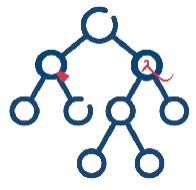
\includegraphics[height=1.0cm]{msca_logo.png}}%
    \end{center}

    \vspace{0.6cm}

    % Main title with Q logos on sides (with clickable links)
    \begin{center}
        \begin{minipage}{0.1\textwidth}
            \centering
            \href{https://quantlet.com}{
\includegraphics[height=1.1cm]{ql_logo.png}}
        \end{minipage}%
        \begin{minipage}{0.78\textwidth}
            \centering
            {\LARGE\bfseries\usebeamercolor[fg]{title}\inserttitle}

            \vspace{0.3cm}

            {\usebeamerfont{subtitle}\usebeamercolor[fg]{title}\insertsubtitle}
        \end{minipage}%
        \begin{minipage}{0.1\textwidth}
            \centering
            \href{https://quantinar.com}{
\includegraphics[height=1.1cm]{qr_logo.png}}
        \end{minipage}
    \end{center}

    \vspace{0.6cm}

    % Authors (left aligned)
    \hspace{0.5cm}{\usebeamerfont{author}\insertauthor}

    \vspace{0.3cm}

    % Institute/Affiliations (left aligned)
    \hspace{0.5cm}\begin{minipage}[t]{0.9\textwidth}
        \raggedright\small\insertinstitute
    \end{minipage}
}

%=============================================================================
% THEOREM ENVIRONMENTS
%=============================================================================
\theoremstyle{definition}
\setbeamertemplate{theorems}[numbered]
\ifdefined\atslang
\newtheorem{defn}{Definiție}
\newtheorem{thm}{Teoremă}
\newtheorem{prop}{Propoziție}
\newtheorem{rmk}{Observație}
\else
\newtheorem{defn}{Definition}
\newtheorem{thm}{Theorem}
\newtheorem{prop}{Proposition}
\newtheorem{rmk}{Remark}
\fi

%=============================================================================
% CENTRED MINIPAGE (no extra vertical space)
%=============================================================================
\newenvironment{cminipage}[1]{%
    \par\noindent\hfill\begin{minipage}{#1}\ignorespaces
}{%
    \end{minipage}\hfill\null\par
}

%=============================================================================
% CUSTOM COMMANDS
%=============================================================================
\newcommand{\E}{\mathbb{E}}
\newcommand{\Var}{\text{Var}}
\newcommand{\Cov}{\text{Cov}}
\newcommand{\Corr}{\text{Corr}}
\newcommand{\R}{\mathbb{R}}
\newcommand{\N}{\mathbb{N}}
\newcommand{\Z}{\mathbb{Z}}
\newcommand{\B}{\mathbf{B}}
\newcommand{\imark}{\textcolor{MainBlue}{\textbullet}}
\newcommand{\RMSE}{\text{RMSE}}
\newcommand{\MAE}{\text{MAE}}
\newcommand{\MAPE}{\text{MAPE}}

% Boldface vector/matrix commands (VAR, VECM, state space)
\newcommand{\bY}{\mathbf{Y}}
\newcommand{\bX}{\mathbf{X}}
\newcommand{\bA}{\mathbf{A}}
\newcommand{\bB}{\mathbf{B}}
\newcommand{\bepsilon}{\boldsymbol{\varepsilon}}
\newcommand{\bSigma}{\boldsymbol{\Sigma}}
\newcommand{\bPhi}{\boldsymbol{\Phi}}
\newcommand{\bGamma}{\boldsymbol{\Gamma}}
\newcommand{\bPi}{\boldsymbol{\Pi}}
\newcommand{\bc}{\mathbf{c}}
\newcommand{\balpha}{\boldsymbol{\alpha}}
\newcommand{\bbeta}{\boldsymbol{\beta}}
\newcommand{\bvarepsilon}{\boldsymbol{\varepsilon}}

% Seminar marks
\newcommand{\correct}{\textcolor{Forest}{\checkmark}}
\newcommand{\incorrect}{\textcolor{Crimson}{\texttimes}}
 se definește
%   \newcommand{\coursename}{Advanced Time Series Analysis and Forecasting}          (EN)
%   \newcommand{\coursename}{Analiza avansată a seriilor de timp și previziune}       (RO)  și  \def\atslang{ro}
% Fișierele .tex se află în EN/Courses, EN/Seminars, RO/Cursuri, RO/Seminarii (două niveluri sub rădăcină).
% Deck-urile sînt generate de latex/build_chapterN.py / build_seminarN.py (vezi latex/ats_build.py).

\documentclass[9pt, aspectratio=169, t]{beamer}
\providecommand{\coursename}{Advanced Time Series Analysis and Forecasting}

% Ensure content fits on slides
\setbeamersize{text margin left=8mm, text margin right=8mm}
% Smaller institute font (title page)
\setbeamerfont{institute}{size=\footnotesize}

%=============================================================================
% THEME AND STYLE CONFIGURATION
%=============================================================================
\usetheme{default}
% Using default theme for clean header/footer control

% Color Palette (matching Redispatch PDF)
\definecolor{MainBlue}{RGB}{26, 58, 110}
\definecolor{AccentBlue}{RGB}{26, 58, 110}
\definecolor{IDAred}{RGB}{205, 0, 0}
\definecolor{DarkGray}{RGB}{51, 51, 51}
\definecolor{MediumGray}{RGB}{128, 128, 128}
\definecolor{LightGray}{RGB}{248, 248, 248}
\definecolor{VeryLightGray}{RGB}{235, 235, 235}
\definecolor{KeynoteGray}{RGB}{218, 218, 218}
\definecolor{SectionGray}{RGB}{120, 120, 120}
\definecolor{FooterGray}{RGB}{100, 100, 100}
\definecolor{Crimson}{RGB}{220, 53, 69}
\definecolor{Forest}{RGB}{46, 125, 50}
\definecolor{Amber}{RGB}{181, 133, 63}
\definecolor{Orange}{RGB}{230, 126, 34}
\definecolor{Purple}{RGB}{142, 68, 173}

% Gradient background (exact Keynote 315° gradient: white to RGB 218,218,218)
\setbeamertemplate{background}{%
    \begin{tikzpicture}[remember picture, overlay]
        \shade[shading=axis, shading angle=315,
        top color=white, bottom color=KeynoteGray]
        (current page.south west) rectangle (current page.north east);
    \end{tikzpicture}%
}
% Fallback solid color for compatibility
\setbeamercolor{background canvas}{bg=}

\setbeamercolor{palette primary}{bg=MainBlue, fg=white}
\setbeamercolor{palette secondary}{bg=MainBlue!85, fg=white}
\setbeamercolor{palette tertiary}{bg=MainBlue!70, fg=white}
\setbeamercolor{structure}{fg=MainBlue}
\setbeamercolor{title}{fg=IDAred}
\setbeamercolor{frametitle}{fg=IDAred, bg=}
\setbeamercolor{block title}{bg=MainBlue, fg=white}
\setbeamercolor{block body}{bg=VeryLightGray, fg=DarkGray}
\setbeamercolor{block title alerted}{bg=Crimson, fg=white}
\setbeamercolor{block body alerted}{bg=Crimson!8, fg=DarkGray}
\setbeamercolor{block title example}{bg=Forest, fg=white}
\setbeamercolor{block body example}{bg=Forest!8, fg=DarkGray}
\setbeamercolor{item}{fg=MainBlue}

% Footer colors (override Madrid theme blue)
\setbeamercolor{author in head/foot}{fg=FooterGray, bg=}
\setbeamercolor{title in head/foot}{fg=FooterGray, bg=}
\setbeamercolor{date in head/foot}{fg=FooterGray, bg=}
\setbeamercolor{section in head/foot}{fg=FooterGray, bg=}
\setbeamercolor{subsection in head/foot}{fg=FooterGray, bg=}

% Bullet styles (apply everywhere including blocks)
\setbeamertemplate{itemize item}{\color{MainBlue}$\boxdot$}
\setbeamertemplate{itemize subitem}{\color{MainBlue}$\blacktriangleright$}
\setbeamertemplate{itemize subsubitem}{\color{MainBlue}\tiny$\bullet$}
\setbeamertemplate{itemize/enumerate body begin}{\normalsize}
\setbeamertemplate{itemize/enumerate subbody begin}{\normalsize}

% Item spacing - compact style
\setlength{\leftmargini}{10pt}       % Level 1: minimal indent
\setlength{\leftmarginii}{10pt}      % Level 2: minimal additional indent
% Compact list spacing (zero extra space before/after lists in blocks)
\makeatletter
\def\@listi{\leftmargin\leftmargini \topsep 0pt \parsep 0pt \itemsep 0pt}
\def\@listii{\leftmargin\leftmarginii \topsep 0pt \parsep 0pt \itemsep 0pt}
\makeatother

\setbeamertemplate{navigation symbols}{}

%=============================================================================
% CUSTOM HEADLINE
%=============================================================================
\setbeamertemplate{headline}{%
    \vskip10pt%
    \hbox to \paperwidth{%
        \hskip0.5cm%
        {\small\color{FooterGray}\renewcommand{\hyperlink}[2]{##2}\insertsectionhead}%
        \hfill%
        \textcolor{FooterGray}{\small\insertframenumber}%
        \hskip0.5cm%
    }%
    \vskip4pt%
    {\color{FooterGray}\hrule height 0.4pt}%
}

%=============================================================================
% CUSTOM FOOTER
%=============================================================================
\usepackage{fontawesome5}

\setbeamertemplate{footline}{%
    {\color{FooterGray}\hrule height 0.4pt}%
    \vskip4pt%
    \hbox to \paperwidth{%
        \hskip0.5cm%
        \textcolor{FooterGray}{\small\coursename}%
        \hfill%
        \raisebox{-0.1em}{%
            \begin{tikzpicture}[x=0.08em, y=0.08em, line width=0.4pt]
                \draw[FooterGray] (0,3) -- (1,4) -- (2,3.5) -- (3,5) -- (4,4) -- (5,6) -- (6,5.5) -- (7,4) -- (8,5) -- (9,7) -- (10,6) -- (11,5) -- (12,6.5) -- (13,8) -- (14,7) -- (15,6) -- (16,7.5) -- (17,9) -- (18,8) -- (19,7) -- (20,8.5) -- (21,10) -- (22,9) -- (23,8) -- (24,9.5);
            \end{tikzpicture}%
        }%
        \hskip0.5cm%
    }%
    \vskip6pt%
}

%=============================================================================
% PACKAGES
%=============================================================================
\usepackage[utf8]{inputenc}
\DeclareUnicodeCharacter{03B1}{\ensuremath{\alpha}}
\usepackage[T1]{fontenc}
\usepackage{amsmath, amssymb, amsthm}
\usepackage{mathtools}
\usepackage{bm}
\usepackage{tikz}
\usetikzlibrary{arrows.meta, positioning, shapes, calc, decorations.pathreplacing, shadings}
\usepackage{booktabs}
\usepackage{multirow}
\usepackage{array}
\usepackage{graphicx}
\usepackage{animate}
\usepackage{hyperref}
\usepackage{colortbl}
\usepackage{listings}
\lstset{language=Python, basicstyle=\ttfamily\scriptsize, keywordstyle=\color{MainBlue}\bfseries,
  commentstyle=\color{Forest}, stringstyle=\color{Crimson}, breaklines=true,
  frame=none, backgroundcolor=\color{VeryLightGray}, xleftmargin=2mm}
\hypersetup{colorlinks=true, linkcolor=MainBlue, urlcolor=MainBlue}
\graphicspath{{../../logos/}{../../charts/}{../../photos/}}
\usepackage{xcolor}
\hfuzz=2pt  % Suppress tiny overfull warnings (<2pt)
\vfuzz=2pt  % Suppress tiny vertical overfull warnings (<2pt)

%=============================================================================
% QUANTLET COMMANDS
%   \quantlet{<displayed name>}{<url>}       (generic)
%   \atsquantlet{Ch_05}{ATS_ch5_garch}       -> https://github.com/danpele/Advanced-Time-Series/tree/main/Quantlets/Ch_05/ATS_ch5_garch
%   \qlurl{<folder>} is defined per chapter by the generator (Quantlets/Ch_NN/<folder>)
%=============================================================================
\newcommand{\atsrepo}{https://github.com/danpele/Advanced-Time-Series}
\newcommand{\atsqlbase}{https://github.com/danpele/Advanced-Time-Series/tree/main/Quantlets}
\newcommand{\quantlet}[2]{%
    \hfill\href{#2}{%
        \raisebox{-0.15em}{
\includegraphics[height=0.7em]{ql_logo.png}}%
        \textcolor{MainBlue}{\tiny\ #1}%
    }%
}
\newcommand{\atsquantlet}[2]{\quantlet{\detokenize{#2}}{\atsqlbase/#1/#2}}

%=============================================================================
% NOTEBOOKS (Google Colab)
%   \colaburl{notebooks/EN/chapter5_seminar_notebook.ipynb} -> the Colab link of a file in the ATS repo
%   \nb: the chapter notebook (each seminar deck redefines it with \renewcommand)
%=============================================================================
\newcommand{\colaburl}[1]{https://colab.research.google.com/github/danpele/Advanced-Time-Series/blob/main/#1}
\newcommand{\nb}{https://colab.research.google.com/github/danpele/Advanced-Time-Series/tree/main/notebooks/EN}
\newcommand{\nbname}{notebooks/EN}

%=============================================================================
% SLIDE HELPERS (used by the generators; the same as in MFM)
%=============================================================================
% local font size for list bodies (the preamble forces \normalsize)
\newcommand{\itemsize}[1]{\setbeamertemplate{itemize/enumerate body begin}{#1}\setbeamertemplate{itemize/enumerate subbody begin}{#1}}
\newcommand{\intitle}[1]{{\hypersetup{urlcolor=white}#1}}   % white links inside coloured title bars
\newcommand{\imgcap}[1]{{\scriptsize #1}\\[0.5mm]}          % caption under a photo
\newcommand{\imgcredit}[2]{{\tiny\color{FooterGray}\href{#1}{#2}}}   % image credit: source URL, author/licence
\newcommand{\aiprompt}[1]{{\ttfamily\color{MainBlue}#1}}     % a prompt to an AI assistant

%=============================================================================
% SEMINARS: student version by default; the instructor wrapper *_solutions.tex sets \solutionstrue
%=============================================================================
\makeatletter\@ifundefined{ifsolutions}{\expandafter\newif\csname ifsolutions\endcsname}{}\makeatother
\newcommand{\solonly}[1]{\ifsolutions #1\fi}
\newcommand{\propsub}{\ifsolutions\else\framesubtitle{\ifdefined\atslang Rezolvarea se discută la seminar\else Solution discussed in class\fi}\fi}

%=============================================================================
% APPENDIX AND CHAPTER LINKS (latex/appendix_links.py writes the calls; it also re-declares these
% macros before \begin{document}, so the decks compile with or without this preamble block)
%=============================================================================
\providecommand{\atsapplink}[3]{\hypertarget{#2}{}\hyperlink{#1}{\beamergotobutton{#3}}}
\providecommand{\atsappback}[2]{\begin{tikzpicture}[remember picture,overlay]\node[anchor=south east] at ([xshift=-3mm,yshift=7mm]current page.south east){\hyperlink{#1}{\beamerreturnbutton{#2}}};\end{tikzpicture}}
\providecommand{\atschlink}[2]{\href{#1}{#2}}
\providecommand{\atschlinkt}[2]{\href{#1}{\usebeamercolor[fg]{frametitle}#2}}

%=============================================================================
% QUANTINAR COMMAND: link către un curs Quantinar (subiecte avansate)
%=============================================================================
\newcommand{\quantinar}[2]{%
    \href{#2}{%
        \raisebox{-0.15em}{
\includegraphics[height=0.8em]{qr_logo.png}}%
        \textcolor{MainBlue}{\scriptsize\ #1}%
    }%
}

%=============================================================================
% CUSTOM TITLE PAGE
%=============================================================================
\defbeamertemplate*{title page}{hybrid}[1][]
{
    \vspace{0.2cm}
    % Logos row - top header (with clickable links)
    \begin{center}
        \href{https://www.ase.ro}{
\includegraphics[height=1.0cm]{ase_logo.png}}\hspace{0.3cm}%
        \href{https://theida.net}{
\includegraphics[height=1.0cm]{ida_logo.png}}\hspace{0.3cm}%
        \href{https://blockchain-research-center.com}{
\includegraphics[height=1.0cm]{brc_logo.png}}\hspace{0.3cm}%
        \href{https://www.ai4efin.ase.ro}{
\includegraphics[height=1.0cm]{ai4efin_logo.png}}\hspace{0.3cm}%
        \href{https://ipe.ro/new}{
\includegraphics[height=1.0cm]{acad_logo.png}}\hspace{0.3cm}%
        \href{https://www.digital-finance-msca.com}{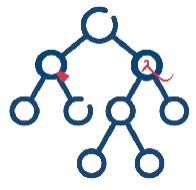
\includegraphics[height=1.0cm]{msca_logo.png}}%
    \end{center}

    \vspace{0.6cm}

    % Main title with Q logos on sides (with clickable links)
    \begin{center}
        \begin{minipage}{0.1\textwidth}
            \centering
            \href{https://quantlet.com}{
\includegraphics[height=1.1cm]{ql_logo.png}}
        \end{minipage}%
        \begin{minipage}{0.78\textwidth}
            \centering
            {\LARGE\bfseries\usebeamercolor[fg]{title}\inserttitle}

            \vspace{0.3cm}

            {\usebeamerfont{subtitle}\usebeamercolor[fg]{title}\insertsubtitle}
        \end{minipage}%
        \begin{minipage}{0.1\textwidth}
            \centering
            \href{https://quantinar.com}{
\includegraphics[height=1.1cm]{qr_logo.png}}
        \end{minipage}
    \end{center}

    \vspace{0.6cm}

    % Authors (left aligned)
    \hspace{0.5cm}{\usebeamerfont{author}\insertauthor}

    \vspace{0.3cm}

    % Institute/Affiliations (left aligned)
    \hspace{0.5cm}\begin{minipage}[t]{0.9\textwidth}
        \raggedright\small\insertinstitute
    \end{minipage}
}

%=============================================================================
% THEOREM ENVIRONMENTS
%=============================================================================
\theoremstyle{definition}
\setbeamertemplate{theorems}[numbered]
\ifdefined\atslang
\newtheorem{defn}{Definiție}
\newtheorem{thm}{Teoremă}
\newtheorem{prop}{Propoziție}
\newtheorem{rmk}{Observație}
\else
\newtheorem{defn}{Definition}
\newtheorem{thm}{Theorem}
\newtheorem{prop}{Proposition}
\newtheorem{rmk}{Remark}
\fi

%=============================================================================
% CENTRED MINIPAGE (no extra vertical space)
%=============================================================================
\newenvironment{cminipage}[1]{%
    \par\noindent\hfill\begin{minipage}{#1}\ignorespaces
}{%
    \end{minipage}\hfill\null\par
}

%=============================================================================
% CUSTOM COMMANDS
%=============================================================================
\newcommand{\E}{\mathbb{E}}
\newcommand{\Var}{\text{Var}}
\newcommand{\Cov}{\text{Cov}}
\newcommand{\Corr}{\text{Corr}}
\newcommand{\R}{\mathbb{R}}
\newcommand{\N}{\mathbb{N}}
\newcommand{\Z}{\mathbb{Z}}
\newcommand{\B}{\mathbf{B}}
\newcommand{\imark}{\textcolor{MainBlue}{\textbullet}}
\newcommand{\RMSE}{\text{RMSE}}
\newcommand{\MAE}{\text{MAE}}
\newcommand{\MAPE}{\text{MAPE}}

% Boldface vector/matrix commands (VAR, VECM, state space)
\newcommand{\bY}{\mathbf{Y}}
\newcommand{\bX}{\mathbf{X}}
\newcommand{\bA}{\mathbf{A}}
\newcommand{\bB}{\mathbf{B}}
\newcommand{\bepsilon}{\boldsymbol{\varepsilon}}
\newcommand{\bSigma}{\boldsymbol{\Sigma}}
\newcommand{\bPhi}{\boldsymbol{\Phi}}
\newcommand{\bGamma}{\boldsymbol{\Gamma}}
\newcommand{\bPi}{\boldsymbol{\Pi}}
\newcommand{\bc}{\mathbf{c}}
\newcommand{\balpha}{\boldsymbol{\alpha}}
\newcommand{\bbeta}{\boldsymbol{\beta}}
\newcommand{\bvarepsilon}{\boldsymbol{\varepsilon}}

% Seminar marks
\newcommand{\correct}{\textcolor{Forest}{\checkmark}}
\newcommand{\incorrect}{\textcolor{Crimson}{\texttimes}}


\newcommand{\qlurl}[1]{https://github.com/danpele/Advanced-Time-Series/tree/main/Quantlets/Ch_04/#1}

% Clickable citations (DOIs verified via Crossref)
\newcommand{\refAL}{\href{https://doi.org/10.1177/1536867X1601600314}{Abrigo și Love (2016)}}
\newcommand{\refBac}{\href{https://doi.org/10.1016/0140-9883(91)90022-R}{Bacon (1991)}}
\newcommand{\refBrP}{\href{https://doi.org/10.1007/978-3-540-75892-1_9}{Breitung și Pesaran (2008)}}
\newcommand{\refCRTa}{\href{https://doi.org/10.1017/S0266466609990776}{Cavaliere, Rahbek și Taylor (2010)}}
\newcommand{\refCRT}{\href{https://doi.org/10.3982/ECTA9099}{Cavaliere, Rahbek și Taylor (2012)}}
\newcommand{\refCP}{\href{https://doi.org/10.1016/j.jeconom.2015.03.007}{Chudik și Pesaran (2015)}}
\newcommand{\refdB}{\href{https://doi.org/10.1111/j.1465-6485.2005.00121.x}{de Bondt (2005)}}
\newcommand{\refECR}{\href{https://doi.org/10.1016/j.jpolmod.2007.01.005}{Égert, Crespo-Cuaresma și Reininger (2007)}}
\newcommand{\refEG}{\href{https://doi.org/10.2307/1913236}{Engle și Granger (1987)}}
\newcommand{\refGN}{\href{https://doi.org/10.1016/S0165-1889(99)00062-7}{Gonzalo și Ng (2001)}}
\newcommand{\refHam}{\href{https://doi.org/10.2307/j.ctv14jx6sm}{Hamilton (1994)}}
\newcommand{\refHNR}{\href{https://doi.org/10.2307/1913103}{Holtz-Eakin, Newey și Rosen (1988)}}
\newcommand{\refIPS}{\href{https://doi.org/10.1016/S0304-4076(03)00092-7}{Im, Pesaran și Shin (2003)}}
\newcommand{\refJohA}{\href{https://doi.org/10.1016/0165-1889(88)90041-3}{Johansen (1988)}}
\newcommand{\refJohB}{\href{https://doi.org/10.2307/2938278}{Johansen (1991)}}
\newcommand{\refJohC}{\href{https://doi.org/10.1111/j.1468-0084.1992.tb00008.x}{Johansen (1992)}}
\newcommand{\refJohD}{\href{https://doi.org/10.1093/0198774508.001.0001}{Johansen (1995a)}}
\newcommand{\refJohE}{\href{https://doi.org/10.1016/0304-4076(94)01664-L}{Johansen (1995b)}}
\newcommand{\refJohF}{\href{https://doi.org/10.1017/S0266466600009026}{Johansen (1995c)}}
\newcommand{\refJohG}{\href{https://doi.org/10.1111/1468-0262.00358}{Johansen (2002)}}
\newcommand{\refJJ}{\href{https://doi.org/10.1111/j.1468-0084.1990.mp52002003.x}{Johansen și Juselius (1990)}}
\newcommand{\refJMN}{\href{https://doi.org/10.1111/1368-423X.00047}{Johansen, Mosconi și Nielsen (2000)}}
\newcommand{\refJus}{\href{https://doi.org/10.1093/oso/9780199285662.001.0001}{Juselius (2006)}}
\newcommand{\refKao}{\href{https://doi.org/10.1016/S0304-4076(98)00023-2}{Kao (1999)}}
\newcommand{\refKPY}{\href{https://doi.org/10.1016/j.jeconom.2010.10.001}{Kapetanios, Pesaran și Yamagata (2011)}}
\newcommand{\refKL}{\href{https://doi.org/10.1017/9781108164818}{Kilian și Lütkepohl (2017)}}
\newcommand{\refKPSW}{\href{https://www.jstor.org/stable/2006644}{King, Plosser, Stock și Watson (1991)}}
\newcommand{\refKS}{\href{https://doi.org/10.1111/obes.12377}{Kripfganz și Schneider (2020)}}
\newcommand{\refLLC}{\href{https://doi.org/10.1016/S0304-4076(01)00098-7}{Levin, Lin și Chu (2002)}}
\newcommand{\refLut}{\href{https://doi.org/10.1007/978-3-540-27752-1}{Lütkepohl (2005)}}
\newcommand{\refMHM}{\href{https://doi.org/10.1002/(SICI)1099-1255(199909/10)14:5\%3C563::AID-JAE530\%3E3.0.CO\%3B2-R}{MacKinnon, Haug și Michelis (1999)}}
\newcommand{\refNar}{\href{https://doi.org/10.1080/00036840500278103}{Narayan (2005)}}
\newcommand{\refNic}{\href{https://doi.org/10.2307/1911408}{Nickell (1981)}}
\newcommand{\refOL}{\href{https://doi.org/10.1111/j.1468-0084.1992.tb00013.x}{Osterwald-Lenum (1992)}}
\newcommand{\refPan}{\href{https://doi.org/10.1017/S0266466600012421}{Pantula (1989)}}
\newcommand{\refPedA}{\href{https://doi.org/10.1111/1468-0084.0610s1653}{Pedroni (1999)}}
\newcommand{\refPedB}{\href{https://doi.org/10.1162/003465301753237803}{Pedroni (2001)}}
\newcommand{\refPedC}{\href{https://doi.org/10.1017/S0266466604203073}{Pedroni (2004)}}
\newcommand{\refPesA}{\href{https://doi.org/10.1111/j.1468-0262.2006.00692.x}{Pesaran (2006)}}
\newcommand{\refPesB}{\href{https://doi.org/10.1002/jae.951}{Pesaran (2007)}}
\newcommand{\refPesC}{\href{https://doi.org/10.1080/07474938.2014.956623}{Pesaran (2015a)}}
\newcommand{\refPesD}{\href{https://doi.org/10.1093/acprof:oso/9780198736912.001.0001}{Pesaran (2015b)}}
\newcommand{\refPesE}{\href{https://doi.org/10.1007/s00181-020-01875-7}{Pesaran (2021)}}
\newcommand{\refPSa}{\href{https://doi.org/10.1017/CCOL0521633230.011}{Pesaran și Shin (1998)}}
\newcommand{\refPSSa}{\href{https://doi.org/10.1080/01621459.1999.10474156}{Pesaran, Shin și Smith (1999)}}
\newcommand{\refPSSb}{\href{https://doi.org/10.1002/jae.616}{Pesaran, Shin și Smith (2001)}}
\newcommand{\refPSm}{\href{https://doi.org/10.1016/0304-4076(94)01644-F}{Pesaran și Smith (1995)}}
\newcommand{\refPH}{\href{https://doi.org/10.2307/2297545}{Phillips și Hansen (1990)}}
\newcommand{\refPM}{\href{https://doi.org/10.1111/1468-0262.00070}{Phillips și Moon (1999)}}
\newcommand{\refRA}{\href{https://doi.org/10.1111/j.1467-9892.1992.tb00113.x}{Reinsel și Ahn (1992)}}
\newcommand{\refSai}{\href{https://doi.org/10.1017/S0266466600004217}{Saikkonen (1991)}}
\newcommand{\refSYG}{\href{https://doi.org/10.1007/978-1-4899-8008-3_9}{Shin, Yu și Greenwood-Nimmo (2014)}}
\newcommand{\refSWa}{\href{https://doi.org/10.2307/2951763}{Stock și Watson (1993)}}
\newcommand{\refSwe}{\href{https://doi.org/10.1111/j.1468-0262.2006.00723.x}{Swensen (2006)}}
\newcommand{\refTY}{\href{https://doi.org/10.1016/0304-4076(94)01616-8}{Toda și Yamamoto (1995)}}
\newcommand{\refWes}{\href{https://doi.org/10.1111/j.1468-0084.2007.00477.x}{Westerlund (2007)}}

\title[Analiza avansată a seriilor de timp și previziune]{Analiza avansată a seriilor de timp și previziune}
\subtitle{Capitolul 4: Cointegrare: VECM, ARDL și date panel}
\author[D.T. Pele]{Daniel Traian PELE}
\institute{Academia de Studii Economice din București\\
IDA Institute Digital Assets\\
Blockchain Research Center\\
AI4EFin Artificial Intelligence for Energy Finance\\
Academia Română, Institutul de Prognoză Economică\\
MSCA Digital Finance}
\date{}

%=============================================================================
\providecommand{\atsapplink}[3]{\hypertarget{#2}{}\hyperlink{#1}{\beamergotobutton{#3}}}  % APPLINKS-MACROS
\providecommand{\atsappback}[2]{\begin{tikzpicture}[remember picture,overlay]\node[anchor=south east] at ([xshift=-3mm,yshift=7mm]current page.south east){\hyperlink{#1}{\beamerreturnbutton{#2}}};\end{tikzpicture}}  % APPLINKS-MACROS
\providecommand{\atschlink}[2]{\href{#1}{#2}}  % APPLINKS-MACROS
\providecommand{\atschlinkt}[2]{\href{#1}{\usebeamercolor[fg]{frametitle}#2}}  % APPLINKS-MACROS
\begin{document}
%=============================================================================

{
\setbeamertemplate{headline}{}
\setbeamertemplate{footline}{}
\begin{frame}[noframenumbering]
    \titlepage
\end{frame}
}
% BEGIN-ACRONYMS (generat de latex/acronyms.py; nu editati manual)
\begin{frame}{Acronime folosite în acest material (1/3)}
\setbeamertemplate{itemize/enumerate body begin}{\tiny}
\begin{columns}[T]
\begin{column}{0.49\textwidth}
\begin{itemize}\setlength{\itemsep}{0pt}
    \item \textbf{ADF}: Augmented Dickey–Fuller (test) — testul Dickey–Fuller augmentat
    \item \textbf{AI}: Artificial Intelligence (inteligență artificială)
    \item \textbf{AIC}: Akaike Information Criterion (criteriul informațional Akaike)
    \item \textbf{AR}: AutoRegressive (model); in event studies: Abnormal Return (model autoregresiv; în studiile de eveniment: randament anormal)
    \item \textbf{ARDL}: AutoRegressive Distributed Lag (model) — model autoregresiv cu decalaje distribuite
    \item \textbf{B230RC0Q173SBEA}: US resident population, quarterly (FRED series code) — populația rezidentă a SUA, trimestrial (codul seriei în FRED)
    \item \textbf{BCE}: Banca Centrală Europeană
    \item \textbf{BIC}: Bayesian Information Criterion (criteriul informațional bayesian (Schwarz))
    \item \textbf{BNR}: Banca Națională a României
    \item \textbf{CADF}: Cross-sectionally augmented Dickey–Fuller (regression) — regresia Dickey–Fuller augmentată cu medii pe secțiune
    \item \textbf{CCE}: Common Correlated Effects (estimator) — estimatorul efectelor comune corelate
    \item \textbf{CCEMG}: Common Correlated Effects Mean Group (estimatorul mean group cu efecte comune corelate)
    \item \textbf{CD}: Cross-section Dependence (test of Pesaran) — testul Pesaran de dependență între unități
\end{itemize}
\end{column}
\begin{column}{0.49\textwidth}
\begin{itemize}\setlength{\itemsep}{0pt}
    \item \textbf{CIPS}: Cross-sectionally augmented IPS (test) — testul IPS augmentat cu medii pe secțiune
    \item \textbf{COVID-19}: COronaVIrus Disease 2019 (boala provocată de coronavirus, 2019)
    \item \textbf{CS-ARDL}: Cross-Sectionally augmented ARDL (ARDL augmentat cu medii pe secțiune)
    \item \textbf{DOLS}: Dynamic Ordinary Least Squares (metoda celor mai mici pătrate dinamică (cu avansuri și decalaje))
    \item \textbf{ECE}: Europa Centrală și de Est
    \item \textbf{ECM}: Error Correction Model (model cu corecția erorii)
    \item \textbf{FE}: Fixed Effects (efecte fixe)
    \item \textbf{FEVD}: Forecast Error Variance Decomposition (descompunerea varianței erorii de prognoză)
    \item \textbf{FMI}: Fondul Monetar Internațional
    \item \textbf{FMOLS}: Fully Modified Ordinary Least Squares (metoda celor mai mici pătrate complet modificată)
    \item \textbf{FPI}: Fixed Private Investment (FRED series code) — investițiile private fixe (codul seriei în FRED)
    \item \textbf{FRED}: Federal Reserve Economic Data (baza de date economice a Rezervei Federale din St. Louis)
    \item \textbf{GARCH}: Generalised AutoRegressive Conditional Heteroskedasticity (heteroscedasticitate condiționată autoregresivă generalizată)
\end{itemize}
\end{column}
\end{columns}
\end{frame}
\begin{frame}{Acronime folosite în acest material (2/3)}
\setbeamertemplate{itemize/enumerate body begin}{\tiny}
\begin{columns}[T]
\begin{column}{0.49\textwidth}
\begin{itemize}\setlength{\itemsep}{0pt}
    \item \textbf{GDP}: Gross Domestic Product (produsul intern brut)
    \item \textbf{GDPDEF}: GDP implicit price deflator (FRED series code) — deflatorul implicit al PIB (codul seriei în FRED)
    \item \textbf{GMM}: Generalized Method of Moments (metoda generalizată a momentelor)
    \item \textbf{HICP}: Harmonised Index of Consumer Prices (indicele armonizat al prețurilor de consum (IAPC))
    \item \textbf{HQ}: Hannan–Quinn (information criterion) — criteriul informațional Hannan–Quinn
    \item \textbf{IAPC}: Indicele armonizat al prețurilor de consum
    \item \textbf{IFS}: International Financial Statistics (IMF) — statisticile financiare internaționale (FMI)
    \item \textbf{IPS}: Im–Pesaran–Shin (panel unit-root test) — testul Im–Pesaran–Shin de rădăcină unitară în panel
    \item \textbf{KPSW}: King–Plosser–Stock–Watson (common-trends model, 1991) — modelul cu trenduri comune King–Plosser–Stock–Watson (1991)
    \item \textbf{LLC}: Levin–Lin–Chu (panel unit-root test) — testul Levin–Lin–Chu de rădăcină unitară în panel
    \item \textbf{LLM}: Large Language Model (model lingvistic de mari dimensiuni)
    \item \textbf{LR}: Likelihood Ratio (test) — testul raportului de verosimilitate
    \item \textbf{MG}: Mean Group (estimator) — estimatorul mean group (media estimațiilor pe unități)
\end{itemize}
\end{column}
\begin{column}{0.49\textwidth}
\begin{itemize}\setlength{\itemsep}{0pt}
    \item \textbf{ML}: Machine Learning (învățare automată)
    \item \textbf{NARDL}: Nonlinear AutoRegressive Distributed Lag (model) — model autoregresiv neliniar cu decalaje distribuite
    \item \textbf{OCDE}: Organizația pentru Cooperare și Dezvoltare Economică
    \item \textbf{OLS}: Ordinary Least Squares (metoda celor mai mici pătrate)
    \item \textbf{PCESV}: Personal Consumption Expenditures: SerVices (FRED series code) — cheltuielile de consum pentru servicii (codul seriei în FRED)
    \item \textbf{PCND}: Personal Consumption expenditures: NonDurable goods (FRED series code) — cheltuielile de consum pentru bunuri nedurabile (codul seriei în FRED)
    \item \textbf{PIB}: Produsul intern brut
    \item \textbf{PMG}: Pooled Mean Group (estimator) — estimatorul pooled mean group (termen lung comun, termen scurt eterogen)
    \item \textbf{PPP}: Purchasing Power Parity (paritatea puterii de cumpărare)
    \item \textbf{PSS}: Pesaran–Shin–Smith (Pesaran–Shin–Smith)
    \item \textbf{RA}: Reinsel–Ahn (small-sample correction) — corecția Reinsel–Ahn pentru eșantioane mici
    \item \textbf{ROBOR}: Romanian Interbank Offer Rate (rata dobînzii interbancare la care se oferă depozite în lei)
    \item \textbf{SE}: Standard Error (eroare standard)
\end{itemize}
\end{column}
\end{columns}
\end{frame}
\begin{frame}{Acronime folosite în acest material (3/3)}
\setbeamertemplate{itemize/enumerate body begin}{\tiny}
\begin{columns}[T]
\begin{column}{0.49\textwidth}
\begin{itemize}\setlength{\itemsep}{0pt}
    \item \textbf{SUA}: Statele Unite ale Americii
    \item \textbf{TSA}: Time Series Analysis (Serii de timp, cursul de licență)
    \item \textbf{UE}: Uniunea Europeană
    \item \textbf{UE-27}: cele 27 de state membre ale Uniunii Europene
    \item \textbf{VAR}: Vector AutoRegression (model vector autoregresiv)
    \item \textbf{VECM}: Vector Error Correction Model (model vectorial cu corecția erorii)
\end{itemize}
\end{column}
\begin{column}{0.49\textwidth}
\end{column}
\end{columns}
\end{frame}
% END-ACRONYMS

\begin{frame}{Întrebarea de azi și traseul}
\itemsize{\small}
\begin{itemize}
    \item \textbf{Întrebarea}: cînd au serii nestaționare un echilibru comun pe termen lung, ce restricții asupra lui putem testa și cît ne putem baza pe răspuns în eșantioane de 100--300 de observații sau pentru 27 de țări?
    \begin{itemize}
        \item cointegrarea este o afirmație despre verosimilitatea unui VAR de rang redus; inferența asupra ei este nestandard și fragilă
    \end{itemize}
    \item \textbf{Traseul} capitolului
    \begin{itemize}
        \item VAR-ul cointegrat ca problemă de verosimilitate; cele cinci cazuri deterministe; corecții pentru eșantioane mici și bootstrap
        \item identificarea și testele asupra lui $\beta$ și $\alpha$; transmiterea dobînzilor în România; I(2) pe scurt; trendurile comune
        \item ARDL și testul bounds; rădăcini unitare și cointegrare în panel; estimatori pentru panele eterogene
    \end{itemize}
    \item Pornim de la \atschlink{https://danpele.github.io/Time-Series-Analysis/RO/Cursuri/capitol7_cointegrare_vecm.pdf}{TSA, Capitolul 7} (Engle--Granger, ECM, VECM, testele Johansen, pairs trading) și de la \atschlink{https://danpele.github.io/Advanced-Time-Series/RO/Cursuri/capitol3_modele_var_structurale_proiectii_locale.pdf}{Capitolul 3} (identificarea structurală); Seminarul 4 are loc înaintea acestui curs
\end{itemize}
\end{frame}

\begin{frame}{Rezultatele învățării}
\itemsize{\small}
\begin{itemize}
    \item Derivați estimatorul Johansen ca regresie de rang redus, enunțați distribuția asimptotică a statisticii trace și alegeți cazul determinist
    \item Corectați testul de rang în eșantioane mici (Reinsel--Ahn, Bartlett, bootstrap wild) și raportați sensibilitatea rangului la numărul de decalaje
    \item Identificați vectorii de cointegrare, testați restricții economice asupra lui $\beta$ și exogenitatea slabă prin $\alpha$ și construiți un VECM structural cu trenduri comune
    \item Aplicați testul bounds ARDL cu valori critice corecte (și pentru eșantioane mici) și alegeți între ARDL și VECM
    \item Testați dependența între unități, rădăcinile unitare și cointegrarea în panel și estimați relațiile de termen lung în panel prin MG, PMG și CCE
\end{itemize}
\end{frame}

\begin{frame}{Bibliografie, date și instrumente}
\itemsize{\small}
\begin{itemize}
    \item Bibliografia de bază: \refJohD; \refJus; \refKL, cap.~3 și 10; \refPesD, cap.~22--31; \refLut, cap.~6--9
    \begin{itemize}
        \item lucrările originale: \refJohA, \refJohB, \refPSSb, \refPSSa, \refPesA, \refPesB; sinteză: \refBrP
    \end{itemize}
    \item Quantlet-urile Python ale capitolului: \href{https://github.com/danpele/Advanced-Time-Series/tree/main/Quantlets/Ch_04}{Quantlets/Ch\_04}
    \begin{itemize}
        \item Johansen în cinci cazuri, ML cu restricții, teste de rang bootstrap, ARDL bounds, LLC/IPS/CIPS, Pedroni, Westerlund, MG, PMG și CCE scrise explicit în \texttt{numpy}
    \end{itemize}
    \item Notebook-ul cursului: \href{\colaburl{notebooks/EN/chapter4_lecture_notebook.ipynb}}{deschideți în Google Colab}
\end{itemize}
\end{frame}

\begin{frame}{Datele folosite în acest capitol}
\itemsize{\footnotesize}
\begin{center}
\scriptsize
\begin{tabular}{>{\raggedright\arraybackslash}p{4.9cm}>{\raggedright\arraybackslash}p{4.6cm}>{\raggedright\arraybackslash}p{2.4cm}}
\toprule
\textbf{Seria} & \textbf{Sursa} & \textbf{Utilizare} \\
\midrule
dobînzile la credite și la depozite în lei; ROBOR 3M & FMI, International Financial Statistics (date BNR); Eurostat irt\_st\_m & VECM, ARDL \\
consumul SUA de bunuri nedurabile și servicii, investițiile fixe, PIB, deflatorul, populația & FRED (PCND, PCESV, FPI, GDP, GDPDEF, B230RC0Q173SBEA) & trenduri comune \\
IAPC România, lunar & Eurostat prc\_hicp\_minr & I(2) \\
UE-27: consumul gospodăriilor, venitul disponibil, deflatorul consumului, populația & Eurostat nama\_10\_gdp, nasa\_10\_nf\_tr, nama\_10\_pe & panel \\
\bottomrule
\end{tabular}
\end{center}
\begin{itemize}
    \item Toate sursele sînt publice și nu cer cont sau cheie; dobînzile lunare pînă în martie 2026, datele SUA pînă în 2025, datele anuale UE pînă în 2024
    \item IAPC (HICP): indicele armonizat al prețurilor de consum; consumul și venitul includ instituțiile fără scop lucrativ în serviciul gospodăriilor
\end{itemize}
\end{frame}

\begin{frame}{De la regresii false la o teorie a verosimilității}
\itemsize{\footnotesize}
\begin{columns}[T]
\begin{column}{0.36\textwidth}
\centering
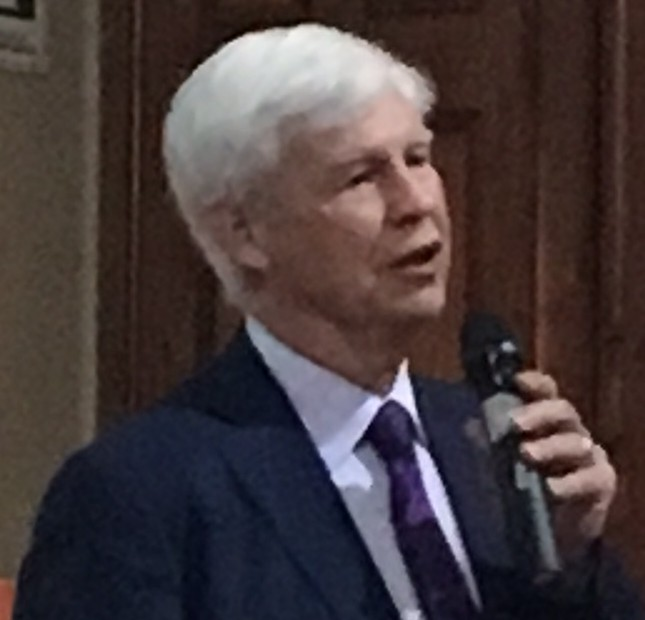
\includegraphics[height=0.36\textheight]{ch4_engle_2017.jpg}\\[1mm]
\imgcap{Robert Engle, 2017}
\imgcredit{https://commons.wikimedia.org/wiki/File:Robert_Engle_SantiagoWEAI2017.png}{Foto: Econterms (2017); CC BY-SA 4.0; Wikimedia Commons}
\end{column}
\begin{column}{0.62\textwidth}
\begin{itemize}
    \item 1987: \refEG\ definesc cointegrarea și demonstrează teorema de reprezentare; estimarea este o regresie în doi pași
    \item 1988--1991: \refJohA\ și \refJohB\ o transformă în verosimilitate maximă pentru un VAR de rang redus: mai multe relații, teste asupra coeficienților lor
    \item 1999--2001: Pesaran, Shin și Smith adaugă testele bounds ARDL \refPSSb\ și panelurile cu coeficienți comuni \refPSSa
    \item 2003: Engle și Granger primesc Premiul Nobel; Granger „pentru metode de analiză a seriilor de timp economice cu trenduri comune (cointegrare)”
    \item De atunci: teste de rang bootstrap, dependența între unități în panel, factori comuni
\end{itemize}
\end{column}
\end{columns}
\end{frame}


%=============================================================================
\section{VAR-ul cointegrat ca problemă de verosimilitate}
%=============================================================================

\begin{frame}{De la TSA la acest capitol}
\itemsize{\small}
\begin{itemize}
    \item Cunoscut (\atschlink{https://danpele.github.io/Time-Series-Analysis/RO/Cursuri/capitol7_cointegrare_vecm.pdf}{TSA, Capitolul 7}): $y_t \sim$ I(1), $\beta'y_t \sim$ I(0); metoda Engle--Granger în doi pași; ECM; $\Pi = \alpha\beta'$; testele trace și max-eigenvalue cu valori critice tabelate
    \item Nou aici
    \begin{itemize}
        \item de ce problema de valori proprii este estimatorul de verosimilitate maximă și cum arată distribuția ei limită
        \item ce caz determinist folosim și ce nu merge în eșantioane de 100--300 de luni
        \item restricții asupra lui $\beta$ (ipoteze economice) și asupra lui $\alpha$ (exogenitate slabă); șocuri structurale cu efecte permanente
        \item ecuații individuale (ARDL) și panele de țări atunci cînd abordarea de sistem cere prea mult
    \end{itemize}
\end{itemize}
\end{frame}

\begin{frame}{VECM și ipoteza $H(r)$}
\itemsize{\small}
\begin{itemize}
    \item $\Delta y_t = \Pi y_{t-1} + \sum_{i=1}^{p-1}\Gamma_i\Delta y_{t-i} + \Phi D_t + \varepsilon_t$, $\varepsilon_t \sim$ i.i.d. $N(0, \Omega)$, $y_t \in \R^n$
    \item $H(r)$: $\Pi = \alpha\beta'$ cu $\alpha, \beta$ de dimensiune $n\times r$; modelele sînt imbricate, $H(0) \subset H(1) \subset \dots \subset H(n)$
    \begin{itemize}
        \item $H(n)$: VAR nerestricționat în niveluri; $H(0)$: VAR în diferențe
        \item doar $\Pi$ este identificat: $\alpha\beta' = (\alpha\xi)(\beta\xi^{-1\prime})'$ pentru orice matrice inversabilă $\xi$ de $r\times r$
    \end{itemize}
    \item $\beta$: cele $r$ relații de cointegrare (termenul lung); $\alpha$: coeficienții de ajustare; $\Gamma_i$: dinamica pe termen scurt
    \item Verosimilitate gaussiană condiționată de primele $p$ observații: estimatorul este ML, testele sînt rapoarte de verosimilitate \refJohA, \refJohB
\end{itemize}
\end{frame}

\begin{frame}{Pasul 1: eliminarea dinamicii pe termen scurt}
\itemsize{\small}
\begin{itemize}
    \item Regresăm $\Delta y_t$ și $y_{t-1}$ pe $Z_{2t} = (\Delta y_{t-1}', \dots, \Delta y_{t-p+1}', D_t')'$; păstrăm reziduurile $R_{0t}$ și $R_{1t}$ (Frisch--Waugh)
    \item Modelul concentrat este o regresie cu un coeficient de rang redus: $R_{0t} = \alpha\beta'R_{1t} + \hat\varepsilon_t$
    \item Matricele de momente $S_{ij} = T^{-1}\sum_t R_{it}R_{jt}'$, $i, j \in \{0, 1\}$
    \item Pentru $\beta$ fixat, OLS a lui $R_{0t}$ pe $\beta'R_{1t}$:
    \begin{itemize}
        \item $\hat\alpha(\beta) = S_{01}\beta(\beta'S_{11}\beta)^{-1}$, $\hat\Omega(\beta) = S_{00} - S_{01}\beta(\beta'S_{11}\beta)^{-1}\beta'S_{10}$
        \item $L_{\max}^{-2/T}(\beta) \propto |\hat\Omega(\beta)|$: rămîne o problemă doar în $\beta$
    \end{itemize}
\end{itemize}
\end{frame}

\begin{frame}{Pasul 2: problema de valori proprii}
\itemsize{\small}
\begin{itemize}
    \item Identitatea determinanților: $|\hat\Omega(\beta)| = |S_{00}|\,\dfrac{|\beta'(S_{11} - S_{10}S_{00}^{-1}S_{01})\beta|}{|\beta'S_{11}\beta|}$
    \item Minimizarea acestui raport de forme pătratice este problema generalizată de valori proprii $|\lambda S_{11} - S_{10}S_{00}^{-1}S_{01}| = 0$, $1 > \hat\lambda_1 > \dots > \hat\lambda_n > 0$
    \item $\hat\beta$ = vectorii proprii $\hat v_1, \dots, \hat v_r$, normalizați prin $\hat\beta'S_{11}\hat\beta = I_r$; atunci $L_{\max}^{-2/T} = |S_{00}|\prod_{i=1}^r(1 - \hat\lambda_i)$
    \item $\hat\lambda_i$ sînt corelațiile canonice la pătrat dintre $R_{0t}$ și $R_{1t}$: un $\hat\lambda_i$ mare = o combinație liniară de niveluri care prezice modificările
    \item O singură descompunere în valori proprii dă estimațiile ML pentru toate valorile lui $r$ deodată (demonstrația: \atsapplink{atsapp1}{atssrc1}{Anexa})
\end{itemize}
\end{frame}

\begin{frame}{Teste de raport de verosimilitate pentru rang}
\itemsize{\small}
\begin{itemize}
    \item \textbf{Trace}: $H(r)$ față de $H(n)$: $LR_{tr}(r) = -T\sum_{i=r+1}^{n}\ln(1 - \hat\lambda_i)$
    \item \textbf{Valoarea proprie maximă}: $H(r)$ față de $H(r + 1)$: $LR_{\max}(r) = -T\ln(1 - \hat\lambda_{r+1})$
    \item Limita sub $H(r)$: $LR_{tr} \Rightarrow \mathrm{tr}\{\int_0^1 (dB)F'(\int_0^1 FF'du)^{-1}\int_0^1 F(dB)'\}$, $B$ o mișcare browniană standard de dimensiune $n - r$
    \begin{itemize}
        \item $F = B$ corectat pentru termenii determiniști ai cazului; limita depinde doar de $n - r$ și de caz, nu de $\alpha, \beta, \Gamma_i, \Omega$
        \item o distribuție Dickey--Fuller multivariată: cuantilele se obțin prin simulare \refOL, \refMHM
    \end{itemize}
    \item Determinarea rangului: testăm pe rînd $r = 0, 1, \dots$ și ne oprim la prima nerespingere; această secvență este consistentă pentru rangul adevărat la un nivel fixat \refJohD
\end{itemize}
\end{frame}

\begin{frame}{Teorema de reprezentare Granger}
\itemsize{\footnotesize}
\begin{columns}[T]
\begin{column}{0.30\textwidth}
\centering
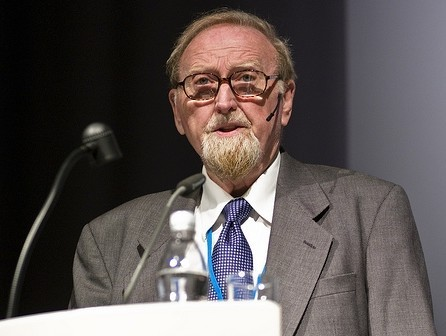
\includegraphics[height=0.33\textheight]{ch1_granger_2008.jpg}\\[1mm]
\imgcap{Clive Granger, 2008}
\imgcredit{https://commons.wikimedia.org/wiki/File:Clive_Granger_by_Olaf_Storbeck.jpg}{Foto: Olaf Storbeck (2008); CC BY-SA 2.0; Wikimedia Commons}
\end{column}
\begin{column}{0.68\textwidth}
\begin{itemize}
    \item Condiții: rădăcinile lui $|A(z)| = 0$ satisfac $|z| > 1$ sau $z = 1$; $\mathrm{rang}\,\Pi = r$; $\alpha_\perp'\Gamma\beta_\perp$ are rang complet, $\Gamma = I - \sum_i\Gamma_i$
    \item Atunci $y_t = C\sum_{i=1}^{t}(\varepsilon_i + \Phi D_i) + C^*(L)(\varepsilon_t + \Phi D_t) + A_0$, cu $C = \beta_\perp(\alpha_\perp'\Gamma\beta_\perp)^{-1}\alpha_\perp'$
    \item $\beta'C = 0$: relațiile nu conțin trendurile stochastice; $C\alpha = 0$: o eroare de echilibru nu are efect permanent
    \item Trenduri comune: cele $n - r$ mersuri aleatoare $\alpha_\perp'\sum_i\varepsilon_i$; $\alpha_\perp'\Gamma\beta_\perp$ singulară înseamnă I(2) (vezi secțiunea despre I(2))
\end{itemize}
\end{column}
\end{columns}
\end{frame}

\begin{frame}{Recapitulare: VAR-ul cointegrat}
\itemsize{\small}
\begin{itemize}
    \item Eliminăm dinamica pe termen scurt, apoi maximizăm după $\beta$: o problemă generalizată de valori proprii
    \item Valorile proprii sînt corelații canonice la pătrat; statisticile trace și max-eigenvalue sînt rapoarte de verosimilitate
    \item Limitele lor sînt funcționale browniene care depind doar de $n - r$ și de termenii determiniști
    \item Reprezentarea Granger: $C = \beta_\perp(\alpha_\perp'\Gamma\beta_\perp)^{-1}\alpha_\perp'$ leagă $\alpha, \beta$ de trendurile comune
\end{itemize}
\end{frame}


%=============================================================================
\section{Termenii determiniști}
%=============================================================================

\begin{frame}{Cinci moduri de a plasa constanta și trendul}
\itemsize{\small}
\begin{itemize}
    \item $\mu_t = \mu_0 + \mu_1t$ cu $\mu_j = \alpha\rho_j + \alpha_\perp\gamma_j$: partea $\alpha$ stă în relații, partea $\alpha_\perp$ antrenează nivelurile \refJohD
    \item \begin{center}
\scriptsize
\begin{tabular}{clll}
\toprule
\textbf{Cazul} & \textbf{Restricția} & \textbf{Nivelurile $y_t$} & \textbf{Relațiile $\beta'y_t$} \\
\midrule
1 ($H_2$) & $\mu_0 = \mu_1 = 0$ & fără drift & medie zero \\
2 ($H_1^*$) & $\mu_0 = \alpha\rho_0$, $\mu_1 = 0$ & fără drift & constantă \\
3 ($H_1$) & $\mu_1 = 0$ & trend liniar & constantă \\
4 ($H^*$) & $\mu_1 = \alpha\rho_1$ & trend liniar & trend liniar \\
5 ($H$) & niciuna & trend pătratic & trend liniar \\
\bottomrule
\end{tabular}
\end{center}

    \item Termenii „restricționați” intră în $Z_{1t}$ alături de $y_{t-1}$ (fac parte din $\beta$); cei „nerestricționați” intră în $Z_{2t}$ și sînt eliminați prin concentrare
    \item Dobînzi: cazul 2; agregate macro cu trend: cazul 3 sau 4; cazul 5 este rar plauzibil
\end{itemize}
\end{frame}

\begin{frame}{Cazul schimbă distribuția sub ipoteza nulă}
\itemsize{\footnotesize}
\begin{center}
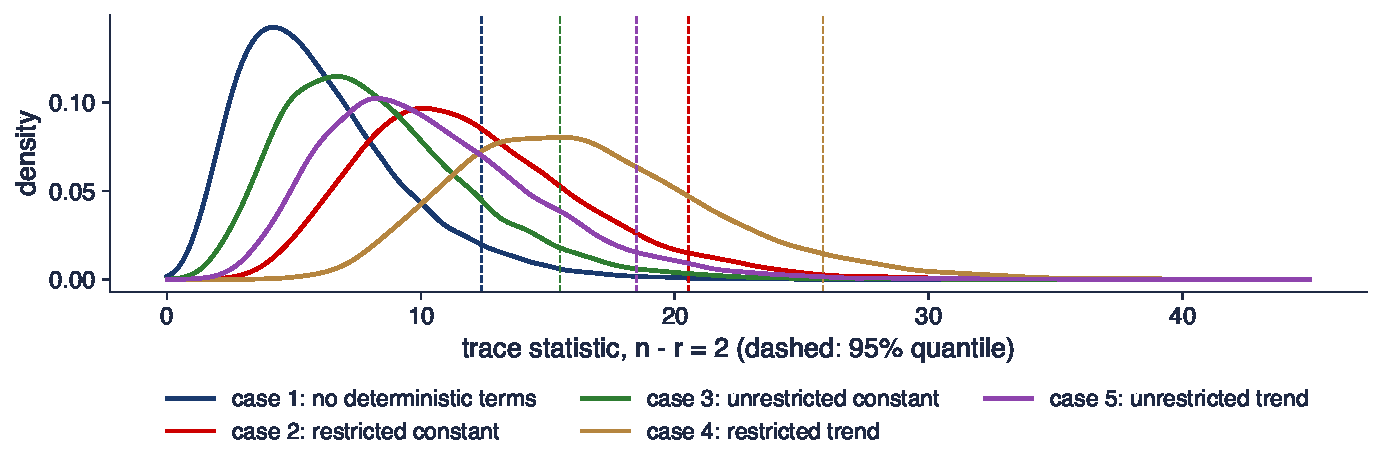
\includegraphics[width=0.97\textwidth,height=0.5\textheight,keepaspectratio]{ats_ch4_trace_dists.pdf}
\end{center}
\vspace{-0.25cm}
\begin{itemize}
    \item Statistica trace sub $H(r)$ cu $n - r = 2$, simulată din mersuri aleatoare (10\,000 de replicări, $T = 400$; drift în cazurile 3 și 5)
    \item Cuantilele de 95\%: 12{,}38 (cazul 1), 20{,}53 (2), 15{,}48 (3), 25{,}84 (4), 18{,}50 (5)
\end{itemize}
\quantlet{ATS\_ch4\_johansen\_asymptotics}{\qlurl{ATS_ch4_johansen_asymptotics}}
\end{frame}

\begin{frame}{Interpretarea celor cinci distribuții}
\itemsize{\small}
\begin{itemize}
    \item Fiecare termen determinist restricționat adaugă un regresor problemei de rang redus și deplasează distribuția spre dreapta
    \item Un trend în niveluri (cazurile 3 și 5) face deterministă o direcție a trendului comun: pentru $n - r = 1$ limita este $\chi^2(1)$, cuantila de 95\% 3{,}89
    \item Folosirea valorilor critice ale cazului 3 într-un model al cazului 2 respinge prea des: cuantila de 95\% pentru $n - r = 1$ este 9{,}25 în cazul 2 și 3{,}89 în cazul 3
    \item Cuantilele simulate diferă de tabelele publicate \refMHM\ cu cel mult cîteva zecimi; Quantlet-ul dă toate cazurile și $n - r = 1, \dots, 4$
\end{itemize}
\end{frame}

\begin{frame}{Cuantilele simulate de 95\% ale statisticii trace}
\itemsize{\small}
\begin{center}
\footnotesize
\begin{tabular}{lccccc}
\toprule
$n - r$ & cazul 1 & cazul 2 & cazul 3 & cazul 4 & cazul 5 \\
\midrule
1 & 4{,}21 & 9{,}25 & 3{,}89 & 12{,}58 & 3{,}84 \\
2 & 12{,}38 & 20{,}53 & 15{,}48 & 25{,}84 & 18{,}50 \\
3 & 24{,}44 & 35{,}24 & 29{,}78 & 43{,}14 & 35{,}36 \\
4 & 40{,}29 & 53{,}68 & 47{,}98 & 63{,}85 & 55{,}54 \\
\bottomrule
\end{tabular}
\end{center}
\begin{itemize}
    \item Simulate cu 10\,000 de replicări ale unei regresii de test VAR(1) pe $T = 400$ de observații; valorile critice din suprafețele de răspuns \refMHM\ diferă cu cel mult cîteva zecimi
    \item Alegerea cazului: întîi graficul datelor; dacă ezitați între 2 și 3 (sau între 3 și 4), testați ipoteza comună asupra rangului și a cazului în ordinea principiului Pantula \refPan, \refJohC
    \item Rupturile în termenii determiniști deplasează din nou distribuția: folosiți valorile critice din \refJMN\ pentru trenduri cu rupturi
\end{itemize}
\end{frame}

\begin{frame}{Recapitulare: termenii determiniști}
\itemsize{\small}
\begin{itemize}
    \item Descompunem fiecare termen determinist într-o parte $\alpha$ (în relații) și una $\alpha_\perp$ (în niveluri)
    \item Cele cinci cazuri au cinci distribuții nule diferite; confundarea lor schimbă rangul
    \item Faceți graficul datelor, alegeți cazul pe criterii economice și folosiți principiul Pantula cînd aveți dubii
\end{itemize}
\end{frame}


%=============================================================================
\section{Eșantioane mici: corecții și bootstrap}
%=============================================================================

\begin{frame}{Respingerile excesive ale testului asimptotic}
\itemsize{\small}
\begin{itemize}
    \item Statistica trace estimează $n^2(p - 1)$ parametri pe termen scurt plus termenii determiniști; cu $T = 100$, $n = 3$ și $p = 4$ aceștia consumă o parte mare din informație
    \item Distorsiunea crește cu dinamica pe termen scurt persistentă ($\Gamma_i$ aproape de cercul unitate) și cu rădăcini ale părții staționare apropiate de unu
    \item Trei remedii
    \begin{itemize}
        \item \textbf{Reinsel--Ahn}: înmulțim statistica cu $(T - np)/T$ \refRA; simplu, adesea prea conservator
        \item \textbf{Corecția Bartlett}: $LR_{tr}/(1 + a(\theta)/T)$ cu $\E LR_{tr} \approx f\,(1 + a(\theta)/T)$, $a(\theta)$ derivat analitic \refJohG
        \item \textbf{Bootstrap}: simulăm distribuția nulă din modelul estimat sub $H(r)$ \refSwe, \refCRT
    \end{itemize}
    \item Heteroscedasticitatea condiționată nu schimbă distribuția limită, dar înrăutățește mărimea testului în eșantioane finite \refCRTa: folosiți bootstrap-ul wild
\end{itemize}
\end{frame}

\begin{frame}{Testul de rang bootstrap, pas cu pas}
\itemsize{\small}
\begin{itemize}
    \item 1. Estimăm VECM sub $H(r)$: $\hat\alpha^{(r)}, \hat\beta^{(r)}, \hat\Gamma_i^{(r)}, \hat\Phi^{(r)}$ și reziduurile $\hat\varepsilon_t^{(r)}$
    \item 2. Generăm $\Delta y_t^* = \hat\alpha^{(r)}\hat\beta^{(r)\prime}y_{t-1}^* + \sum_i\hat\Gamma_i^{(r)}\Delta y_{t-i}^* + \hat\Phi^{(r)}D_t + \varepsilon_t^*$ pornind de la valorile inițiale observate
    \item 3. Inovațiile: $\varepsilon_t^* = \hat\varepsilon_t^{(r)}w_t$, $w_t \sim$ i.i.d. $N(0, 1)$ (wild) sau reziduuri reeșantionate (bootstrap i.i.d.)
    \begin{itemize}
        \item varianta wild păstrează tiparul de volatilitate al fiecărei date
    \end{itemize}
    \item 4. Calculăm $LR_{tr}^*(r)$ pe fiecare eșantion; valoarea $p$ = ponderea cazurilor $LR_{tr}^* \ge LR_{tr}(r)$; testăm $r = 0, 1, \dots$ și ne oprim la prima nerespingere
    \item Estimarea sub $H(r)$ (nu sub $H(n)$) este esențială: datele bootstrap trebuie să aibă exact $n - r$ rădăcini unitare \refCRT
\end{itemize}
\end{frame}

\begin{frame}{Mărimea testului de rang în eșantioane mici (simulare)}
\itemsize{\footnotesize}
\begin{center}
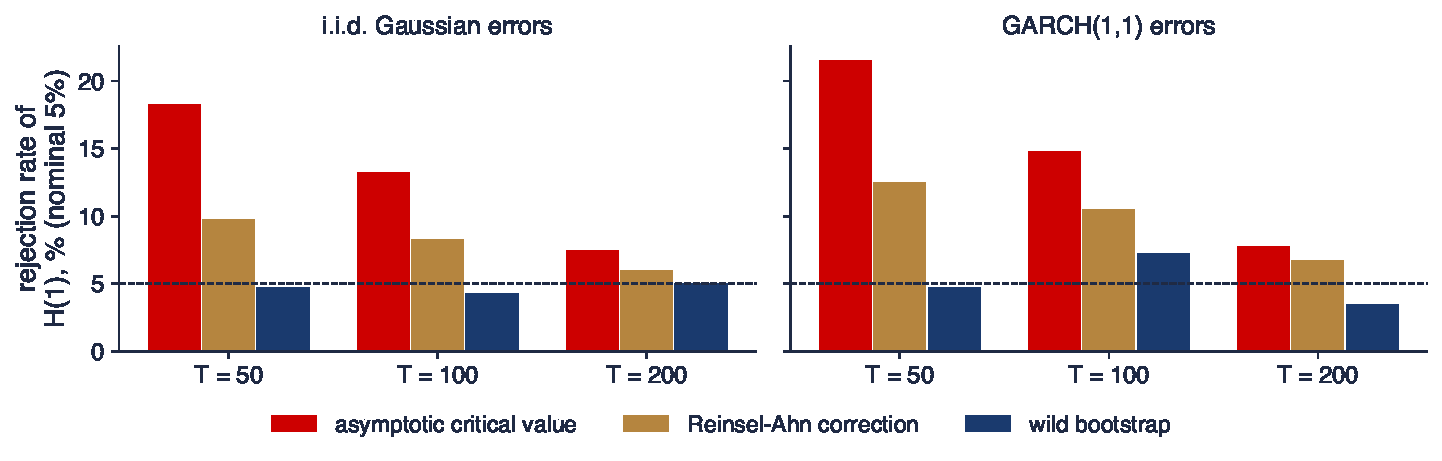
\includegraphics[width=0.97\textwidth,height=0.5\textheight,keepaspectratio]{ats_ch4_size_mc.pdf}
\end{center}
\vspace{-0.25cm}
\begin{itemize}
    \item VECM cu trei variabile, rangul adevărat 1, $\Gamma_1 = 0{,}8I$, cazul 2, VAR(2); testul lui $H(1)$ la 5\%; 400 de replicări, cîte 199 de eșantioane bootstrap
    \item $T = 50$, erori i.i.d.: asimptotic 18{,}2\%, Reinsel--Ahn 9{,}8\%, bootstrap wild 4{,}8\%
\end{itemize}
\quantlet{ATS\_ch4\_johansen\_asymptotics}{\qlurl{ATS_ch4_johansen_asymptotics}}
\end{frame}

\begin{frame}{Interpretarea simulării mărimii testului}
\itemsize{\small}
\begin{itemize}
    \item Cu dinamică persistentă pe termen scurt, testul asimptotic găsește o a doua relație falsă în 18{,}2\% din eșantioanele de 50 și în 13{,}2\% din cele de 100
    \item Reinsel--Ahn înjumătățește distorsiunea; bootstrap-ul wild este aproape de 5\% pentru orice $T$, și cu erori GARCH (4{,}8\% la $T = 50$, asimptotic 21{,}5\%)
    \item La $T = 200$ toate trei sînt acceptabile: problema este raportul dintre numărul de parametri și numărul de observații, nu metoda
    \item În practică: raportați valorile $p$ asimptotice și bootstrap una lîngă alta și rangul pentru numere de decalaje apropiate
\end{itemize}
\end{frame}

\begin{frame}{Recapitulare: eșantioane mici}
\itemsize{\small}
\begin{itemize}
    \item Testul trace asimptotic respinge prea des cînd parametrii sînt mulți și dinamica pe termen scurt este persistentă
    \item Reinsel--Ahn și corecția Bartlett rescalează statistica; bootstrap-ul îi reconstruiește distribuția
    \item Bootstrap din modelul estimat sub $H(r)$; ponderi wild cînd volatilitatea se schimbă în timp
\end{itemize}
\end{frame}


%=============================================================================
\section{Identificarea și testele asupra lui $\beta$ și $\alpha$}
%=============================================================================

\begin{frame}{Normalizarea nu înseamnă identificare}
\itemsize{\small}
\begin{itemize}
    \item Vectorii proprii dau o bază a spațiului de cointegrare $\mathrm{sp}(\beta)$; orice $\beta\xi$ generează același spațiu și descrie datele la fel de bine
    \item Împărțirea fiecărui vector la un coeficient fixează scala ($r$ restricții), dar nu și rotația: mai sînt necesare $r(r - 1)$ restricții, cîte $r - 1$ pentru fiecare vector
    \item Restricții liniare vector cu vector: $\beta = (H_1\varphi_1, \dots, H_r\varphi_r)$, $H_i$ de dimensiune $n_1\times s_i$, $R_i = H_{i\perp}$
    \begin{itemize}
        \item condiția de rang \refJohE: pentru orice $i$ și orice mulțime de $k$ alți vectori, $\mathrm{rang}(R_i'(H_{i_1}, \dots, H_{i_k})) \ge k$, $k = 1, \dots, r - 1$
        \item este analogul condiției de rang din sistemele de ecuații simultane; condiția de ordin singură nu este suficientă
    \end{itemize}
    \item Identificarea este economie: fiecare restricție este o afirmație de tipul „pe termen lung, dobînda la credite nu depinde de dobînda la depozite”
\end{itemize}
\end{frame}

\begin{frame}{Testarea restricțiilor asupra lui $\beta$}
\itemsize{\small}
\begin{itemize}
    \item \textbf{Aceeași restricție pentru toți vectorii}, $\beta = H\varphi$ ($H$: $n_1\times s$): rezolvăm $|\lambda H'S_{11}H - H'S_{10}S_{00}^{-1}S_{01}H| = 0$
    \begin{itemize}
        \item $LR = T\sum_{i=1}^r\ln\{(1 - \tilde\lambda_i)/(1 - \hat\lambda_i)\} \to \chi^2(r(n_1 - s))$; de exemplu, excluderea unei variabile din toate relațiile
    \end{itemize}
    \item \textbf{Restricții diferite pe vectori}, $\beta = (H_1\varphi_1, \dots, H_r\varphi_r)$: fără formă închisă; maximizăm $-\tfrac{T}{2}\ln|\hat\Omega(\beta)|$ prin algoritmul de comutare sau numeric
    \begin{itemize}
        \item restricții de supraidentificare: $LR \to \chi^2(\sum_i(n_1 - r + 1 - s_i))$
    \end{itemize}
    \item $\beta$ \textbf{complet cunoscut} (de exemplu, raporturile mari): $LR = T\{\ln|\hat\Omega(\beta_0)| - \ln|S_{00}| - \sum_{i\le r}\ln(1 - \hat\lambda_i)\} \to \chi^2(r(n_1 - r))$
    \item Pentru un rang dat, $\hat\beta$ este superconsistent și mixt gaussian: testele LR asupra lui $\beta$ sînt $\chi^2$, spre deosebire de testul de rang \refJohB
\end{itemize}
\end{frame}

\begin{frame}{Restricții asupra lui $\alpha$ și exogenitatea slabă}
\itemsize{\small}
\begin{itemize}
    \item $\alpha = A\psi$ ($A$: $n\times m$): condiționăm sistemul pe $A_\perp'R_{0t}$ și rezolvăm problema de valori proprii a celor $m$ ecuații rămase; $LR = T\sum_{i\le r}\ln\{(1 - \tilde\lambda_i)/(1 - \hat\lambda_i)\} \to \chi^2(r(n - m))$
    \item \textbf{Exogenitatea slabă} a lui $x_t$ pentru $\beta$: rîndul lui $\alpha$ corespunzător lui $x_t$ este zero ($r$ restricții)
    \begin{itemize}
        \item $x_t$ nu se ajustează la dezechilibrele trecute; este un trend comun (o coloană a lui $\alpha_\perp$)
        \item atunci modelul condiționat al lui $\Delta y_t$ dat $\Delta x_t$ este complet eficient pentru $\beta$: baza ECM și ARDL pe o singură ecuație
    \end{itemize}
    \item Ipotezele structurale de termen lung sînt restricții comune asupra lui $\beta$ și $\alpha$
    \begin{itemize}
        \item PPP: $(1, -1, -1)$ pentru (preț, preț extern, curs de schimb); Fisher: $(1, -1)$ pentru (dobîndă, inflație); transmitere completă: $(1, -1)$ pentru (dobînda bancară, dobînda de politică sau de piață)
    \end{itemize}
\end{itemize}
\end{frame}

\begin{frame}{Recapitulare: identificarea și testele}
\itemsize{\small}
\begin{itemize}
    \item Identificați $\beta$ cu cîte $r - 1$ restricții motivate economic pe vector; verificați condiția de rang
    \item Pentru un rang dat, testele LR asupra lui $\beta$ și $\alpha$ sînt $\chi^2$ cu grade de libertate cunoscute
    \item Un rînd zero al lui $\alpha$ = exogenitate slabă = permisiunea de a condiționa pe acea variabilă
\end{itemize}
\end{frame}


%=============================================================================
\section{Aplicație: transmiterea dobînzilor în România}
%=============================================================================

\begin{frame}{Cît de repede și cît de complet urmează băncile ROBOR?}
\itemsize{\footnotesize}
\begin{columns}[T]
\begin{column}{0.36\textwidth}
\centering

\includegraphics[height=0.34\textheight]{ch0_bnr_palace_2015.jpg}\\[1mm]
\imgcap{Palatul BNR, București}
\imgcredit{https://commons.wikimedia.org/wiki/File:Bucharest_-_BNR_Palace_(19644434340).jpg}{Foto: Ștefan Jurcă (2015); CC BY 2.0; Wikimedia Commons}
\end{column}
\begin{column}{0.62\textwidth}
\begin{itemize}
    \item Politica monetară ajunge la gospodării și firme doar prin dobînzile bancare; ROBOR 3M este referința pentru majoritatea creditelor în lei cu dobîndă variabilă
    \item Zona euro: transmiterea pe termen lung către dobînzile la credite este adesea completă, către cele la depozite incompletă \refdB; ECE: transmitere mai rapidă și mai completă după prima parte a tranziției \refECR
    \item Ipoteze: $H_\beta$: pe termen lung, dobînzile la credite și la depozite se mișcă unu la unu cu ROBOR; $H_\alpha$: ROBOR nu se ajustează la dobînzile bancare
    \item Date: august 2005 -- martie 2026, $T = 248$ de luni (perioada țintirii inflației)
\end{itemize}
\end{column}
\end{columns}
\end{frame}

\begin{frame}{Dobînda la credite, dobînda la depozite și ROBOR 3M}
\itemsize{\footnotesize}
\begin{center}
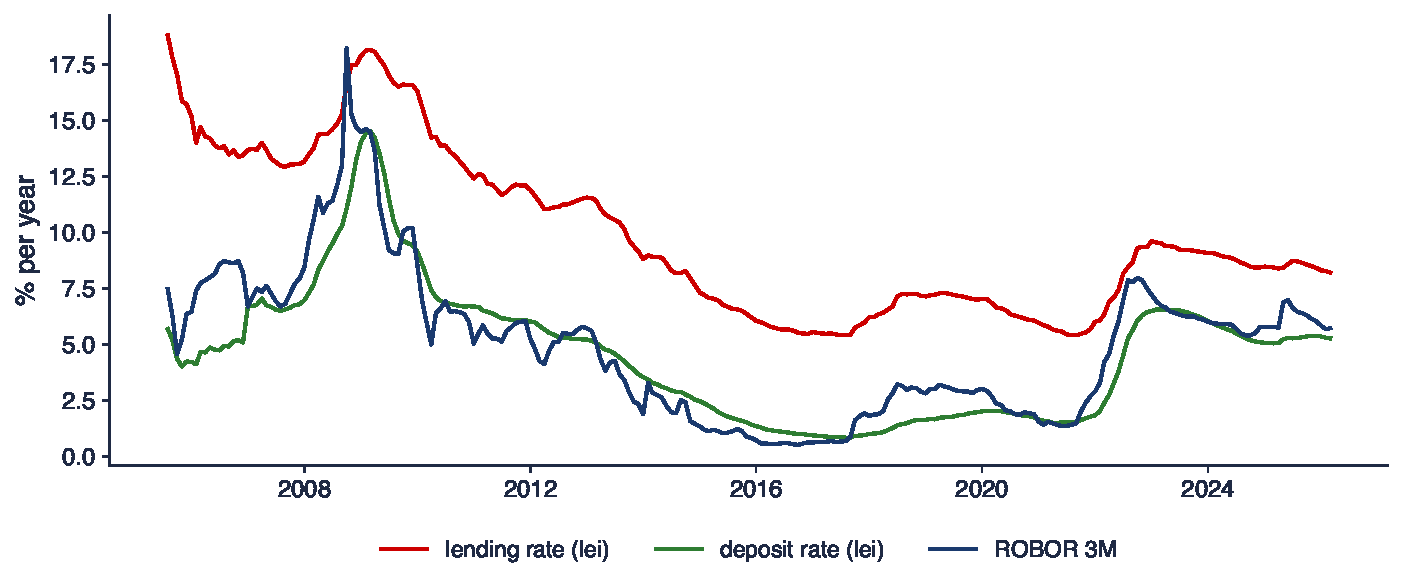
\includegraphics[width=0.97\textwidth,height=0.5\textheight,keepaspectratio]{ats_ch4_rates.pdf}
\end{center}
\vspace{-0.25cm}
\begin{itemize}
    \item Lunar, \% pe an; dobînzile la credite și la depozite în lei (FMI IFS, raportate de BNR); ROBOR 3M (Eurostat)
    \item ROBOR variază între 0{,}51\% și 18{,}2\%; diferența dintre dobînda la credite și ROBOR scade de la 11{,}3 pp la 2{,}5 pp
\end{itemize}
\quantlet{ATS\_ch4\_passthrough\_vecm}{\qlurl{ATS_ch4_passthrough_vecm}}
\end{frame}

\begin{frame}{Interpretarea celor trei dobînzi}
\itemsize{\small}
\begin{itemize}
    \item Toate trei se îndepărtează mult de orice medie în douăzeci de ani: le tratăm ca I(1) în eșantion, chiar dacă dobînzile sînt mărginite teoretic
    \item Se mișcă împreună după 2008, în 2014--2015 și în 2022: argumentul vizual pentru cointegrare
    \item Scăderea diferenței în 2005--2010 este finalul tranziției (concurență, prime de risc în scădere), nu un efect al politicii monetare
    \item Un trend în niveluri nu este plauzibil pentru dobînzi: cazul 2, constanta restricționată la relații
\end{itemize}
\end{frame}

\begin{frame}{Rangul sistemului de transmitere}
\itemsize{\small}
\begin{center}
\scriptsize
\begin{tabular}{lccccccc}
\toprule
$H(r)$ & $LR_{tr}$ & RA & cv 5\% & wild $p$ & $LR_{tr}$, $p{=}4$ & RA, $p{=}4$ & wild $p$, $p{=}4$ \\
\midrule
$r = 0$ & 121{,}1 & 118{,}1 & 35{,}2 & 0{,}007 & 40{,}0 & 38{,}0 & 0{,}647 \\
$r \le 1$ & 52{,}2 & 50{,}9 & 20{,}5 & 0{,}022 & 14{,}9 & 14{,}1 & 0{,}812 \\
$r \le 2$ & 4{,}3 & 4{,}2 & 9{,}3 & 0{,}767 & 3{,}8 & 3{,}6 & 0{,}820 \\
\bottomrule
\end{tabular}
\end{center}
\begin{itemize}
    \item Cazul 2; RA: Reinsel--Ahn; cv: cuantila simulată de 95\%; $p$ wild: 399 de eșantioane bootstrap wild sub $H(r)$; numărul de decalaje după BIC = 2, HQ = 5, AIC = 8
    \item Cu $p = 2$ toate cele trei metode dau $r = 2$; cu $p = 4$ testul asimptotic dă $r = 1$, iar bootstrap-ul wild nu respinge nimic
\end{itemize}
\end{frame}

\begin{frame}{Interpretarea testelor de rang}
\itemsize{\small}
\begin{itemize}
    \item Două relații sînt exact ceea ce prezice teoria: una pentru dobînzile la credite, una pentru cele la depozite, ambele ancorate de ROBOR
    \item Rezultatul este fragil: două decalaje în plus și o inferență robustă la heteroscedasticitate elimină dovezile; volatilitatea din 2008--2009 domină eșantionul
    \item Continuăm cu $r = 2$ pentru că teoria și modelul parcimonios coincid și raportăm sensibilitatea
    \item Un rang ales astfel este o decizie de modelare, nu o măsurătoare: enunțați-o înainte de a testa restricțiile
\end{itemize}
\end{frame}

\begin{frame}{Relațiile identificate și testele}
\itemsize{\small}
\begin{itemize}
    \item Exact identificate (o excludere pe vector): $\text{credit}_t = 1{,}13\,\text{ROBOR}_t + 3{,}62$, $\text{depozit}_t = 0{,}93\,\text{ROBOR}_t + 0{,}09$
    \item Ajustarea: dobînda la credite $\alpha_{11} = \ensuremath{-}0{,}056$ (la propria relație), dobînda la depozite $\alpha_{22} = \ensuremath{-}0{,}071$; ROBOR: 0{,}014 și 0{,}017
    \item \begin{center}
\scriptsize
\begin{tabular}{lccc}
\toprule
\textbf{Ipoteza} & $LR$ & gl & $p$ \\
\midrule
transmitere completă către ambele dobînzi & 8{,}98 & 2 & 0{,}011 \\
transmitere completă către dobînda la credite & 4{,}16 & 1 & 0{,}041 \\
ROBOR slab exogen (rînd zero în $\alpha$) & 0{,}57 & 2 & 0{,}752 \\
\bottomrule
\end{tabular}
\end{center}

    \item Cu $p = 4$: transmiterea către credite 1{,}11, valoarea $p$ pentru transmiterea completă către credite 0{,}458, pentru exogenitatea slabă 0{,}819
\end{itemize}
\end{frame}

\begin{frame}{Cele două erori de echilibru}
\itemsize{\footnotesize}
\begin{center}
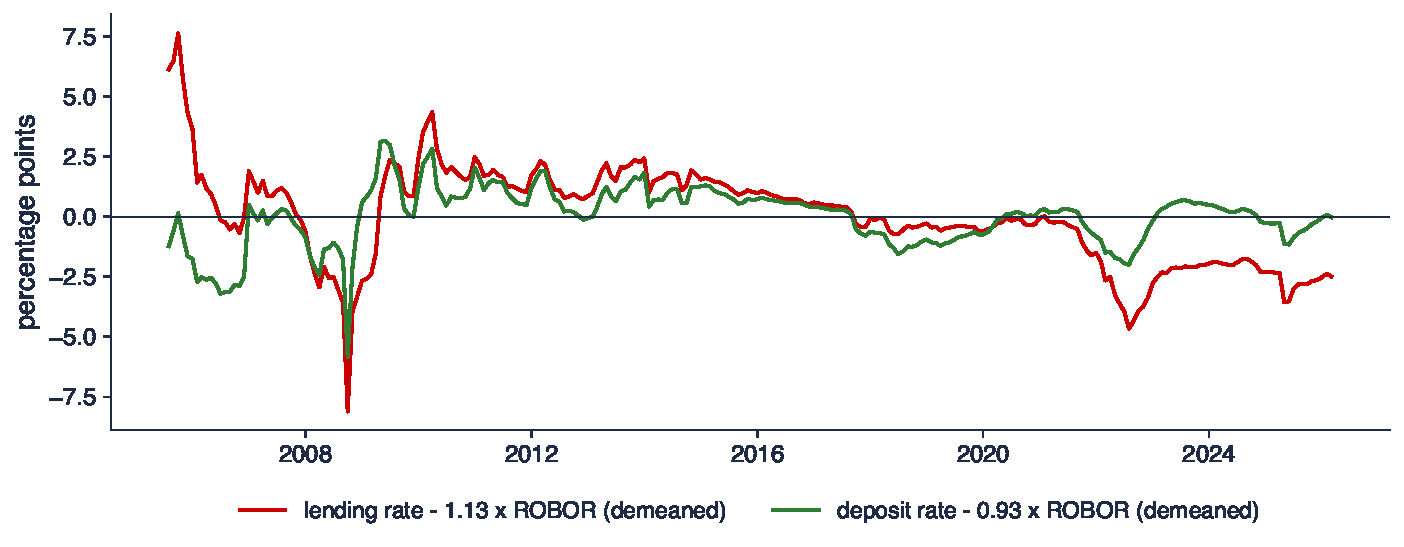
\includegraphics[width=0.97\textwidth,height=0.52\textheight,keepaspectratio]{ats_ch4_pt_ect.pdf}
\end{center}
\vspace{-0.25cm}
\begin{itemize}
    \item $\hat\beta_i'y_t$ pentru relațiile exact identificate, centrate; ar trebui să arate staționar dacă rangul și $\beta$ sînt corecte
\end{itemize}
\quantlet{ATS\_ch4\_passthrough\_vecm}{\qlurl{ATS_ch4_passthrough_vecm}}
\end{frame}

\begin{frame}{Interpretarea VECM-ului de transmitere}
\itemsize{\small}
\begin{itemize}
    \item Dobînzile la credite reacționează ușor peste unu pe termen lung (1{,}13 pentru un punct de ROBOR), cele la depozite sub unu (0{,}93): marja băncilor crește cînd crește ROBOR
    \item Transmiterea completă comună este respinsă ($p = 0{,}011$), din cauza depozitelor; pentru dobînzile la credite verdictul depinde de numărul de decalaje
    \item ROBOR este slab exogen ($p = 0{,}752$): dobînzile pieței monetare conduc, dobînzile bancare urmează; aceasta justifică un ARDL pe o singură ecuație
    \item Eroarea de echilibru pentru credite este persistentă înainte de 2010: diferența din perioada tranziției nu este o marjă stabilă, un candidat pentru o constantă cu ruptură \refJMN
\end{itemize}
\end{frame}

\begin{frame}{Recapitulare: transmiterea în România}
\itemsize{\small}
\begin{itemize}
    \item Două relații de cointegrare cu ROBOR ca trend comun, dar rangul este sensibil la decalaje și la heteroscedasticitate
    \item Transmiterea către credite este apropiată de unu (ușor peste), cea către depozite sub unu
    \item Exogenitatea slabă a lui ROBOR nu este respinsă: un model condiționat pe o singură ecuație este legitim
\end{itemize}
\end{frame}


%=============================================================================
\section{I(2) pe scurt}
%=============================================================================

\begin{frame}{Cînd modelul I(1) nu este suficient}
\itemsize{\small}
\begin{itemize}
    \item Dacă $\alpha_\perp'\Gamma\beta_\perp$ are rang redus $s < n - r$, reprezentarea Granger nu mai funcționează: unele trenduri comune sînt I(2), $y_t$ conține $\sum\sum\varepsilon$
    \item Candidați tipici: nivelurile prețurilor și masa monetară nominală în perioade cu inflație variabilă; inflația este atunci I(1)
    \item Modelul I(2): două condiții de rang redus, $\Pi = \alpha\beta'$ și $\alpha_\perp'\Gamma\beta_\perp = \xi\eta'$; ML și teste de rang în \refJohF, ghid aplicat în \refJus
    \begin{itemize}
        \item cointegrare polinomială: $\beta'y_t + \delta'\Delta y_t \sim$ I(0), de exemplu masa monetară reală plus un multiplu al inflației
    \end{itemize}
    \item Verificare practică: testați rădăcina unitară pentru $\Delta y_t$; dacă VECM-ul I(1) are o rădăcină aproape de unu în partea staționară, suspectați I(2); soluția uzuală este modelarea variabilelor reale (deflatate)
\end{itemize}
\end{frame}

\begin{frame}{Este nivelul prețurilor din România I(2)?}
\itemsize{\footnotesize}
\begin{center}
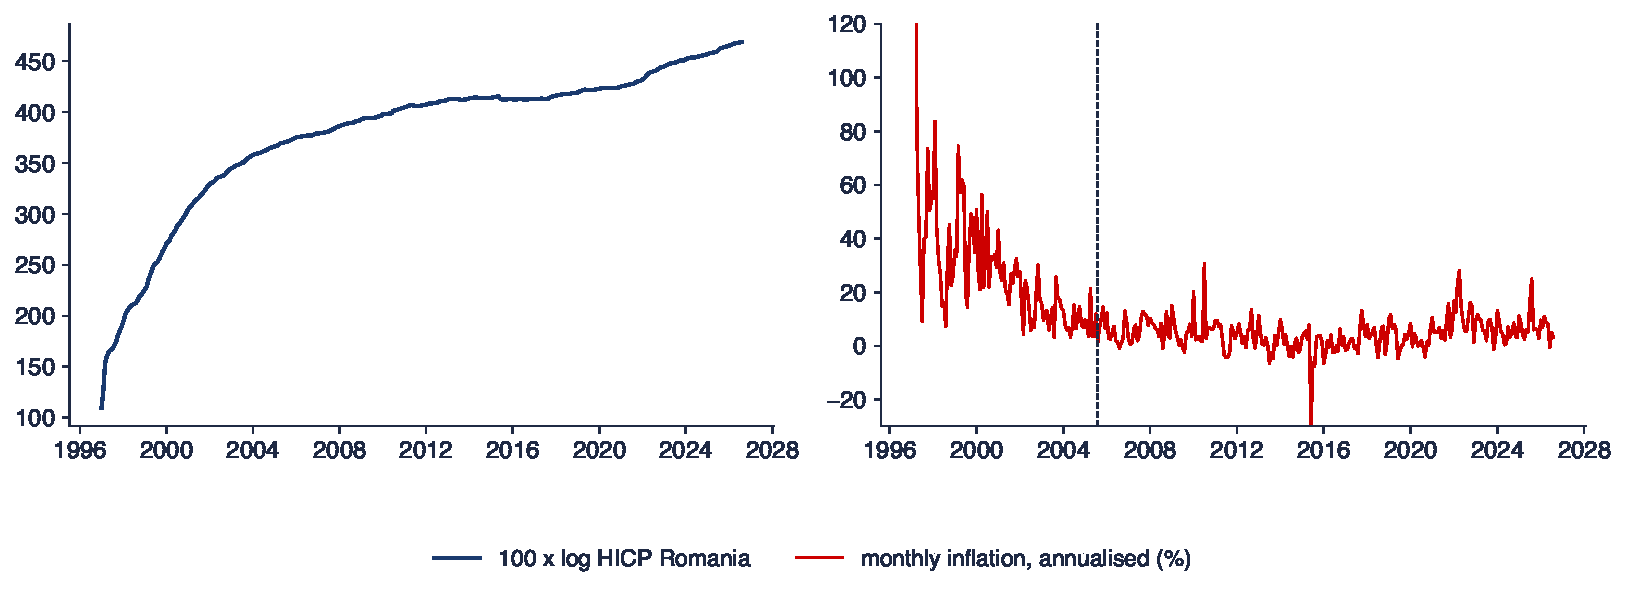
\includegraphics[width=0.97\textwidth,height=0.48\textheight,keepaspectratio]{ats_ch4_i2.pdf}
\end{center}
\vspace{-0.25cm}
\begin{itemize}
    \item Stînga: $100\ln$ IAPC; dreapta: inflația lunară, anualizată; linia punctată: țintirea inflației din august 2005
    \item ADF $t$ pentru inflația lunară (12 decalaje): \ensuremath{-}4{,}25 pentru 1997--2026, \ensuremath{-}2{,}39 din 2005 (valoarea critică 5\%: $-2{,}87$); pentru modificarea ei: \ensuremath{-}6{,}13
\end{itemize}
\quantlet{ATS\_ch4\_i2\_check}{\qlurl{ATS_ch4_i2_check}}
\end{frame}

\begin{frame}{Interpretarea verificării I(2)}
\itemsize{\small}
\begin{itemize}
    \item Pe 1997--2026, dezinflația arată ca revenire la medie, iar inflația apare staționară: nivelul prețurilor este I(1)
    \item Din 2005, o rădăcină unitară în inflație nu este respinsă: în eșantionul țintirii inflației, nivelul prețurilor se comportă ca I(2)
    \item Răspunsul depinde de eșantion, ca și pentru rang: de aceea sistemele cu niveluri nominale se rescriu de obicei în termeni reali și inflație
    \item Sistemul nostru de transmitere folosește dobînzi, cel mult I(1): problema I(2) nu apare acolo
\end{itemize}
\end{frame}


%=============================================================================
\section{VECM structural: trenduri comune}
%=============================================================================

\begin{frame}{Șocuri permanente și tranzitorii}
\itemsize{\small}
\begin{itemize}
    \item Reprezentarea Granger: efectul pe termen lung al lui $\varepsilon_t$ asupra lui $y_{t+h}$, $h \to \infty$, este $C\varepsilon_t$, iar $\mathrm{rang}\,C = n - r$
    \item Cu șocuri structurale $\varepsilon_t = Bu_t$ ($\E u_tu_t' = I$): impactul pe termen lung $CB$ are cel mult $n - r$ coloane nenule: $k = n - r$ șocuri permanente și $r$ tranzitorii
    \item Numărătoarea (în \atschlink{https://danpele.github.io/Advanced-Time-Series/RO/Cursuri/capitol3_modele_var_structurale_proiectii_locale.pdf}{Capitolul 3} erau necesare $n(n - 1)/2$ restricții): cointegrarea dă gratuit $rk$ restricții zero pe termen lung
    \begin{itemize}
        \item mai sînt necesare: $k(k - 1)/2$ între șocurile permanente și $r(r - 1)/2$ între cele tranzitorii \refKL, \refGN
    \end{itemize}
    \item Cu un singur trend comun ($k = 1$), șocul permanent este identificat fără alte ipoteze: $u_t^P = \alpha_\perp'\varepsilon_t/(\alpha_\perp'\Omega\alpha_\perp)^{1/2}$, impactul $b^P = \Omega\alpha_\perp(\alpha_\perp'\Omega\alpha_\perp)^{-1/2}$
    \item Aceasta generalizează Blanchard--Quah (\atschlink{https://danpele.github.io/Advanced-Time-Series/RO/Cursuri/capitol3_modele_var_structurale_proiectii_locale.pdf}{Capitolul 3}): acolo zeroul de termen lung era impus; aici provine din rangul de cointegrare
\end{itemize}
\end{frame}

\begin{frame}{Studiu de caz: King, Plosser, Stock și Watson (1991)}
\itemsize{\small}
\begin{itemize}
    \item \refKPSW: într-un model de ciclu real cu trend stochastic al productivității, consumul, investițiile și producția au un singur trend comun: raporturile mari (great ratios) $c - y$ și $i - y$ sînt staționare
    \begin{itemize}
        \item $n = 3$, $r = 2$, $\beta = \begin{pmatrix}1 & 0\\ 0 & 1\\ -1 & -1\end{pmatrix}$ impus; un singur șoc permanent de „creștere echilibrată”
        \item întrebarea: cît din ciclul economic explică șocul permanent?
    \end{itemize}
    \item Replicarea noastră: date trimestriale SUA 1949T1--1988T4 (eșantionul lucrării), $T = 160$; $c$: bunuri nedurabile și servicii, $i$: investiții fixe, $y$: PIB, pe locuitor, deflatate cu deflatorul PIB
    \begin{itemize}
        \item VAR($2$) în niveluri (toate criteriile), cazul 3; trace: 45{,}8; 19{,}4; 1{,}4 față de cuantilele de 95\% 29{,}8; 15{,}5; 3{,}9: $r = 2$
        \item raporturile mari exacte sînt respinse: $LR = 16{,}6$, $\chi^2(2)$, $p = $<$\,0{,}001$; cu trend restricționat (cazul 4) nu sînt respinse: $LR = 0{,}50$, $p = 0{,}778$
    \end{itemize}
\end{itemize}
\end{frame}

\begin{frame}{Șocul de creștere echilibrată}
\itemsize{\footnotesize}
\begin{center}
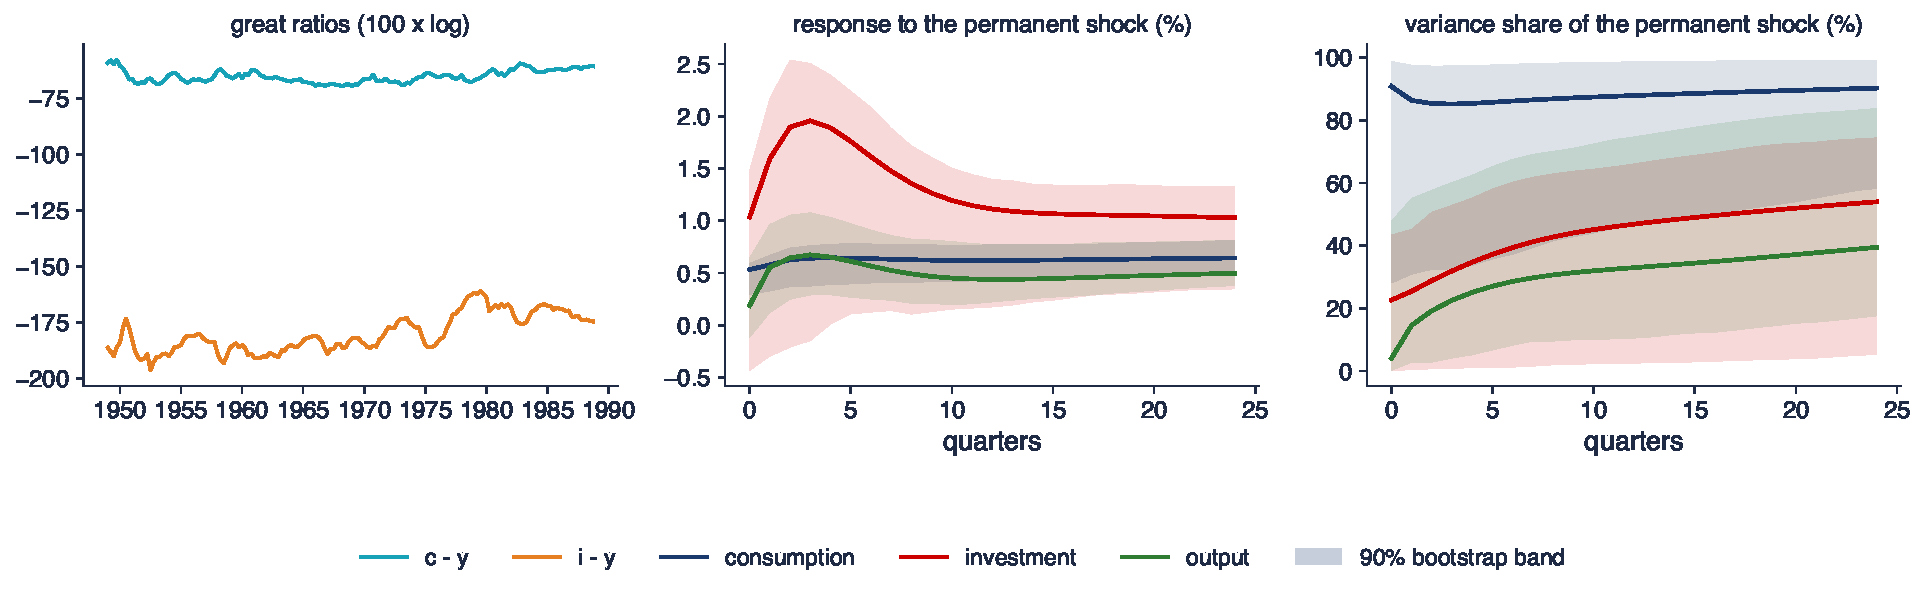
\includegraphics[width=0.97\textwidth,height=0.48\textheight,keepaspectratio]{ats_ch4_kpsw.pdf}
\end{center}
\vspace{-0.25cm}
\begin{itemize}
    \item Raporturile mari impuse (cazul 3); șoc permanent de o abatere standard; benzi bootstrap pe reziduuri de 90\% (300 de eșantioane, $\beta$ fixat)
    \item Efectul pe termen lung 0{,}74\% pentru toate trei; ponderea în varianța producției: 4\% la 1 trimestru, 30\% la 8, 39\% la 24 [17; 83]
\end{itemize}
\quantlet{ATS\_ch4\_common\_trends}{\qlurl{ATS_ch4_common_trends}}
\end{frame}

\begin{frame}{Interpretarea modelului cu trenduri comune}
\itemsize{\small}
\begin{itemize}
    \item Creșterea echilibrată are loc prin construcție pe termen lung: șocul mișcă $c$, $i$ și $y$ cu același 0{,}74\%; investițiile depășesc nivelul final pe termen scurt
    \item Șocul permanent domină consumul (87\% la 8 trimestre, logica venitului permanent), dar explică o minoritate a fluctuațiilor producției la orizonturile ciclului economic
    \item Benzile sînt largi: cu $T = 160$ datele abia separă variația permanentă de cea tranzitorie
    \item Ca în \atschlink{https://danpele.github.io/Advanced-Time-Series/RO/Cursuri/capitol3_modele_var_structurale_proiectii_locale.pdf}{Capitolul 3}, partea economică este ipoteza de identificare: aici, care relații sînt staționare
\end{itemize}
\end{frame}

\begin{frame}{Cît de robust este răspunsul?}
\itemsize{\small}
\begin{center}
\footnotesize
\begin{tabular}{lcccc}
\toprule
\textbf{Specificația} & $h = 1$ & $h = 4$ & $h = 8$ & $h = 24$ \\
\midrule
raporturi mari, cazul 3, 1949--1988 & 4\% & 23\% & 30\% & 39\% \\
raporturi mari cu trend, cazul 4, 1949--1988 & 34\% & 37\% & 52\% & 77\% \\
raporturi mari, cazul 3, 1949--2019 & 51\% & 30\% & 29\% & 40\% \\
raporturi mari, cazul 3, 1949--2025 & 28\% & 20\% & 20\% & 29\% \\
\bottomrule
\end{tabular}
\end{center}
\begin{itemize}
    \item Ponderea șocului permanent în varianța erorii de prognoză a producției, la $h$ trimestre
    \item Permițînd un trend în raporturi (creșterea ponderii serviciilor), rolul șocului permanent crește considerabil la orizonturi scurte; extinderea eșantionului îl schimbă din nou; statistica LR a raporturilor mari crește la 24{,}3 pe date pînă în 2025
    \item Concluzie: importanța „șocurilor de trend” în ciclu nu este determinată doar de date
\end{itemize}
\end{frame}

\begin{frame}{Recapitulare: VECM structural}
\itemsize{\small}
\begin{itemize}
    \item Cointegrarea împarte șocurile în $n - r$ permanente și $r$ tranzitorii și furnizează $rk$ zerouri de termen lung
    \item Cu un singur trend comun, șocul permanent este $\alpha_\perp'\varepsilon_t$, scalat
    \item KPSW: creșterea echilibrată dă o identificare curată, dar ponderile varianței depind de cazul determinist și de eșantion
\end{itemize}
\end{frame}


%=============================================================================
\section{ARDL și testul bounds}
%=============================================================================

\begin{frame}{De la VECM la un ECM condiționat}
\itemsize{\small}
\begin{itemize}
    \item Partiționăm $y_t = (y_t, x_t')'$, $x_t$ de dimensiune $k$; dacă $x_t$ este slab exogen și există o singură relație care îl conține pe $y_t$, modelul condiționat este
    \item $\Delta y_t = c_0 + c_1t + \pi_{yy}y_{t-1} + \pi_{yx}'x_{t-1} + \sum_{i=1}^{p-1}\psi_i\Delta y_{t-i} + \sum_{j=0}^{q-1}\omega_j'\Delta x_{t-j} + u_t$ \refPSSb
    \item Este un ARDL($p, q$) în niveluri, rescris; coeficienții de termen lung $\theta = -\pi_{yx}/\pi_{yy}$, viteza de ajustare $\pi_{yy}$
    \begin{itemize}
        \item OLS este consistent, iar $\hat\theta$ are o limită mixt gaussiană cînd decalajele absorb endogenitatea lui $x_t$ \refPSa
        \item erorile standard ale lui $\hat\theta$ prin metoda delta; testele $t$ asupra lui $\theta$ sînt valabile asimptotic
    \end{itemize}
    \item Avantajul: $x_t$ poate fi I(0), I(1) sau un amestec și nu trebuie testat în prealabil
\end{itemize}
\end{frame}

\begin{frame}{Testul bounds}
\itemsize{\small}
\begin{itemize}
    \item $H_0$: nu există relație în niveluri, $\pi_{yy} = 0$ și $\pi_{yx} = 0$; testul Wald $F$ (și $t$ pentru $\pi_{yy}$, ca să excludem cazul degenerat $\pi_{yy} = 0 \ne \pi_{yx}$)
    \item Distribuția nulă depinde de ordinul de integrare al lui $x_t$: limita inferioară dacă tot $x_t$ este I(0), limita superioară dacă tot este I(1)
    \begin{itemize}
        \item $F$ peste limita superioară: respingem (există relație în niveluri); sub limita inferioară: nu respingem; între ele: neconcludent, iar ordinul de integrare contează
    \end{itemize}
    \item Cinci cazuri (ca la Johansen): I fără termeni; II termen liber restricționat; III termen liber nerestricționat; IV termen liber nerestricționat, trend restricționat; V termen liber și trend nerestricționate
    \begin{itemize}
        \item în cazurile II și IV termenii restricționați fac parte din $H_0$; limitele pentru $t$ există pentru cazurile I, III, V
    \end{itemize}
    \item Limite simulate de 5\% ($T = 1000$, 10\,000 de replicări), $k = 1$: cazul II [3{,}58; 4{,}14], cazul III [4{,}97; 5{,}71]; $t$, cazul III: [\ensuremath{-}2{,}86; \ensuremath{-}3{,}22]
\end{itemize}
\end{frame}

\begin{frame}{Valori critice în eșantioane mici}
\itemsize{\small}
\begin{itemize}
    \item PSS tabelează limite asimptotice ($T = 1000$); cu 30--80 de observații anuale acestea sînt prea mici \refNar
    \item Simularea noastră, cazul III, $k = 1$, 5\%: $T = 30$: [5{,}52; 6{,}32], $T = 80$: [5{,}02; 5{,}86], $T = 250$: [4{,}98; 5{,}73], asimptotic: [4{,}97; 5{,}71]
    \item Regresiile de suprafață de răspuns dau valori critice și valori $p$ aproximative pentru orice $T$, $k$ și număr de decalaje \refKS: folosiți-le în locul tabelului asimptotic
    \item Greșeli frecvente în lucrările aplicate
    \begin{itemize}
        \item cazul greșit (limitele cazului III pentru un model estimat în cazul II); regresori I(2), pentru care limitele nu sînt valabile
        \item feedback de la $y_t$ la $x_t$ (fără exogenitate slabă) sau mai multe relații între variabile
    \end{itemize}
\end{itemize}
\end{frame}

\begin{frame}{ARDL sau VECM?}
\itemsize{\small}
\begin{center}
\scriptsize
\begin{tabular}{>{\raggedright\arraybackslash}p{3.0cm}>{\raggedright\arraybackslash}p{4.4cm}>{\raggedright\arraybackslash}p{4.4cm}}
\toprule
 & \textbf{ARDL} & \textbf{VECM} \\
\midrule
Relații & una, normalizată pe $y_t$ & $r$, rangul estimat \\
Regresori & I(0), I(1) sau amestecați; slab exogeni & toți I(1); toți endogeni \\
Inferență & bounds $F$ și $t$; $\theta$ prin metoda delta & trace/max-eigenvalue; teste $\chi^2$ pentru $\beta$, $\alpha$ \\
Eșantioane mici & puțini parametri; necesită limite pentru eșantioane mici & mulți parametri; necesită bootstrap \\
Utilizare structurală & multiplicatorii lui $x$ asupra lui $y$ & trenduri comune, șocuri identificate \\
\bottomrule
\end{tabular}
\end{center}
\begin{itemize}
    \item Regula: estimați întîi VECM cînd este posibil; dacă o variabilă este slab exogenă și relația este unică, ARDL este eficient și mai simplu; dacă există feedback, estimațiile ARDL sînt inconsistente
\end{itemize}
\end{frame}

\begin{frame}{ARDL: transmiterea ROBOR către dobînda la credite}
\itemsize{\small}
\begin{itemize}
    \item ARDL(4, 2) ales după BIC, cazul II (ROBOR slab exogen în VECM), $n = 244$
    \item Bounds $F = 4{,}27$; limite de 5\% asimptotice [3{,}58; 4{,}14], la $T$-ul nostru [3{,}67; 4{,}14]: există relație în niveluri
    \begin{itemize}
        \item aceeași regresie în cazul III: $F = 5{,}87$ față de [4{,}94; 5{,}79]: neconcludent; $t = \ensuremath{-}3{,}28$ față de [\ensuremath{-}2{,}86; \ensuremath{-}3{,}22]
    \end{itemize}
    \item Transmiterea pe termen lung $\hat\theta = 1{,}15$ (SE 0{,}12): transmiterea completă nu este respinsă de testul $t$; viteza $\hat\pi_{yy} = \ensuremath{-}0{,}026$ (SE 0{,}008), timpul de înjumătățire 27 de luni
    \item Dobînda la depozite: $F = 7{,}68$, $\hat\theta = 0{,}94$ (SE 0{,}05), timpul de înjumătățire 12 luni: incompletă, dar mai rapidă
\end{itemize}
\end{frame}

\begin{frame}{Limitele pentru eșantioane mici și multiplicatorii dinamici}
\itemsize{\footnotesize}
\begin{center}
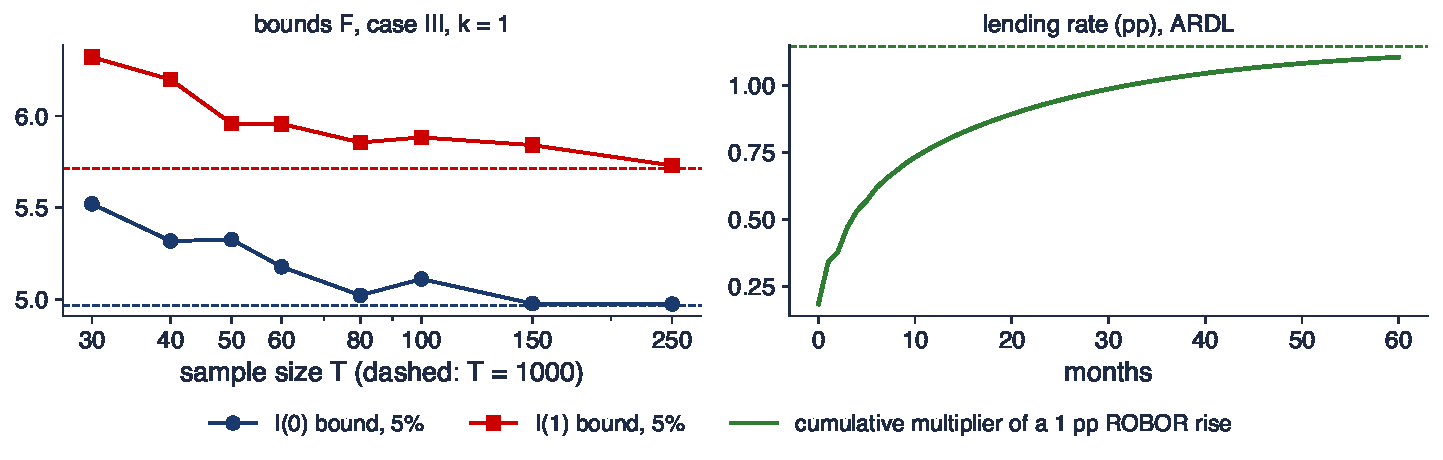
\includegraphics[width=0.97\textwidth,height=0.48\textheight,keepaspectratio]{ats_ch4_bounds.pdf}
\end{center}
\vspace{-0.25cm}
\begin{itemize}
    \item Stînga: limite simulate de 5\%, cazul III, $k = 1$, în funcție de $T$ (punctat: $T = 1000$); dreapta: răspunsul cumulat al dobînzii la credite la o creștere permanentă de 1 pp a ROBOR (punctat: $\hat\theta$)
    \item Multiplicatori: 0{,}18 la impact, 0{,}62 după 6 luni, 0{,}77 după 12, 0{,}94 după 24, 1{,}11 după 60
\end{itemize}
\quantlet{ATS\_ch4\_ardl\_bounds}{\qlurl{ATS_ch4_ardl_bounds}}
\end{frame}

\begin{frame}{Interpretarea rezultatelor ARDL}
\itemsize{\small}
\begin{itemize}
    \item Limita superioară scade de la 6{,}32 la $T = 30$ la 5{,}73 la $T = 250$: cu date anuale tabelul asimptotic respinge prea des
    \item Verdictul asupra relației în niveluri depinde de caz: alegeți cazul II sau III pe criterii economice (dobînzile nu au drift) înainte de a vă uita la $F$
    \item ARDL și VECM coincid asupra mărimii transmiterii către credite (1{,}15 și 1{,}13), dar nu asupra testului $\theta = 1$: alți parametri de perturbare, altă putere
    \item Aproximativ jumătate din efectul de termen lung apare în șase luni (0{,}62); restul este lent, cu un timp de înjumătățire a dezechilibrului de 27 de luni, în acord cu perioadele cu dobîndă fixă și cu reevaluarea contractelor
\end{itemize}
\end{frame}

\begin{frame}{Două instrumente înrudite}
\itemsize{\small}
\begin{itemize}
    \item \textbf{Cauzalitatea Toda--Yamamoto} \refTY: într-un VAR cu variabile posibil integrate sau cointegrate, estimăm $p + d_{\max}$ decalaje în niveluri și testăm doar primele $p$
    \begin{itemize}
        \item statistica Wald este asimptotic $\chi^2(p)$ oricare ar fi proprietățile de integrare și cointegrare; prețul: putere mai mică decît un VECM corect specificat
    \end{itemize}
    \item \textbf{ARDL neliniar} \refSYG: descompunem $x_t$ în sumele parțiale ale creșterilor $x_t^+ = \sum_{j\le t}\max(\Delta x_j, 0)$ și ale scăderilor $x_t^-$
    \begin{itemize}
        \item asimetrie pe termen lung: $\theta^+ \ne \theta^-$; asimetrie pe termen scurt: $\omega_j^\pm$ diferiți; teste Wald, limite cu $k = 2$
        \item utilizarea clasică: prețurile carburanților cresc repede cu petrolul și scad încet („rachete și pene”) \refBac; Seminarul 4 testează acest lucru pentru România
    \end{itemize}
\end{itemize}
\end{frame}

\begin{frame}{Recapitulare: ARDL și testul bounds}
\itemsize{\small}
\begin{itemize}
    \item ECM-ul condiționat este un ARDL rescris; necesită exogenitate slabă și o singură relație
    \item Testul bounds evită testarea prealabilă a regresorilor, cu prețul unei zone neconcludente
    \item Folosiți cazul corect și valori critice pentru eșantioane mici (suprafețe de răspuns)
    \item Toda--Yamamoto pentru cauzalitate fără testare prealabilă; NARDL pentru ajustare asimetrică
\end{itemize}
\end{frame}


%=============================================================================
\section{Serii de timp panel}
%=============================================================================

\begin{frame}{Datele panel: cîștigul și problemele noi}
\itemsize{\footnotesize}
\begin{columns}[T]
\begin{column}{0.30\textwidth}
\centering

\includegraphics[height=0.27\textheight]{ch4_ecb_frankfurt_2015.jpg}\\[1mm]
\imgcap{Sediul BCE, Frankfurt}
\imgcredit{https://commons.wikimedia.org/wiki/File:Seat_of_the_European_Central_Bank_and_Frankfurt_Skyline_at_dawn_20150422_1.jpg}{Foto: DXR (2015); CC BY-SA 4.0; Wikimedia Commons}
\end{column}
\begin{column}{0.68\textwidth}
\begin{itemize}
    \item Seriile pe țări sînt scurte (20--30 de ani de date anuale): un test de rang sau bounds pentru o singură țară are putere mică; $N$ țări adaugă informație
    \item Asimptotică în două dimensiuni: secvențială ($T \to \infty$, apoi $N \to \infty$) sau comună cu $N/T \to 0$; o regresie panel cu serii I(1) estimează o relație medie de termen lung chiar fără cointegrare \refPM, \refKao
    \item Două probleme noi: \textbf{eterogenitatea} (dinamica diferă între țări) și \textbf{dependența între unități} (șocuri comune: recesiunea din 2009, COVID-19, euro)
    \item Testele de primă generație presupun unități independente; cele de generația a doua modelează dependența \refBrP
\end{itemize}
\end{column}
\end{columns}
\end{frame}

\begin{frame}{Măsurarea dependenței între unități}
\itemsize{\small}
\begin{itemize}
    \item Corelațiile pe perechi $\hat\rho_{ij}$ ale reziduurilor (sau ale seriilor centrate); statistica \textbf{CD} \refPesE: $CD = \sqrt{\dfrac{2T}{N(N - 1)}}\sum_{i<j}\hat\rho_{ij} \to N(0, 1)$
    \item Ipoteza nulă este dependența \emph{slabă} \refPesC: o corelație care dispare în medie cînd $N$ crește; un factor comun cu încărcări de medie nenulă dă $|CD| \to \infty$
    \item Valabil pentru $T$ fix și $N$ mare, și în panele dinamice sau cu rădăcini unitare; corelațiile pozitive și negative se pot compensa, deci raportați și media $|\hat\rho_{ij}|$
    \item UE-27, $T = 22$ (2001--2022): CD = 50{,}3 pentru creșterea consumului (media $|\hat\rho| = 0{,}59$), 25{,}7 pentru creșterea venitului, 62{,}4 pentru inflație: dependență puternică peste tot
\end{itemize}
\end{frame}

\begin{frame}{Teste de rădăcină unitară în panel}
\itemsize{\small}
\begin{itemize}
    \item \textbf{LLC} \refLLC: $\Delta y_{it} = \mu_i + \rho y_{i,t-1} + \sum_j\gamma_{ij}\Delta y_{i,t-j} + e_{it}$, $\rho$ comun; $H_1$: toate unitățile staționare cu același $\rho$
    \begin{itemize}
        \item $t$ comun pe reziduuri ortogonalizate și normalizate, ajustat cu media și varianța tabelate
    \end{itemize}
    \item \textbf{IPS} \refIPS: $\rho_i$ eterogeni; $\bar t = N^{-1}\sum_i t_i$ (ADF individuale), $Z = \sqrt N(\bar t - \E t)/\sqrt{\Var t} \to N(0, 1)$
    \begin{itemize}
        \item $H_1$: o fracțiune nenulă de unități este staționară; respingerea nu spune care
    \end{itemize}
    \item \textbf{CIPS} \refPesB: un factor comun $f_t$ în erori; augmentăm fiecare ADF cu $\bar y_{t-1}$ și $\Delta\bar y_{t-j}$ (CADF) și facem media rapoartelor $t$
    \begin{itemize}
        \item mediile pe secțiune aproximează $f_t$; distribuția este nestandard și tabelată
    \end{itemize}
    \item Sub dependență puternică, LLC și IPS resping prea des: tratează 27 de țări corelate ca 27 de dovezi independente
\end{itemize}
\end{frame}

\begin{frame}{Rădăcini unitare în panelul UE-27}
\itemsize{\small}
\begin{center}
\footnotesize
\begin{tabular}{lccc}
\toprule
\textbf{Variabila} & LLC & IPS $\bar t$ & CIPS \\
\midrule
consum (trend) & \ensuremath{-}12{,}85 (0{,}075) & \ensuremath{-}2{,}67 (0{,}003) & \ensuremath{-}2{,}38 (0{,}290) \\
venit (trend) & \ensuremath{-}11{,}82 (0{,}305) & \ensuremath{-}2{,}09 (0{,}660) & \ensuremath{-}2{,}18 (0{,}566) \\
inflație (constantă) & \ensuremath{-}10{,}10 (0{,}003) & \ensuremath{-}1{,}82 (0{,}038) & \ensuremath{-}2{,}36 (0{,}009) \\
\bottomrule
\end{tabular}
\end{center}
\begin{itemize}
    \item $c$, $y$: $100\ln$ consumul real și venitul disponibil real pe locuitor ale gospodăriilor; $\pi$: inflația deflatorului consumului; $N = 27$, $T = 22$, un decalaj
    \item Valorile $p$ în paranteze provin din 1\,000 de simulări ale ipotezei nule cu unități independente, pentru $N$ și $T$ ale noastre (în locul momentelor tabelate)
    \item Consumul: IPS respinge rădăcina unitară ($p = 0{,}003$), CIPS nu ($p = 0{,}290$): „staționaritatea” era un factor comun; inflația este staționară după toate testele
\end{itemize}
\end{frame}

\begin{frame}{Teste de cointegrare în panel}
\itemsize{\small}
\begin{itemize}
    \item \textbf{Pe reziduuri} \refPedA, \refPedC: estimăm $y_{it} = a_i + \delta_it + \beta_i'x_{it} + e_{it}$ țară cu țară și testăm rădăcina unitară a reziduurilor
    \begin{itemize}
        \item șapte statistici: patru „panel” (within, coeficient AR comun) și trei „group” (between, eterogene); $H_0$: nicio unitate nu este cointegrată
        \item impun o restricție de factor comun (dinamica pe termen scurt a lui $x$ și $y$ la fel); \refKao\ este cazul particular omogen
    \end{itemize}
    \item \textbf{Pe ECM} \refWes: $\Delta y_{it} = d_i + \alpha_iy_{i,t-1} + \lambda_i'x_{i,t-1} + \sum_j a_{ij}\Delta y_{i,t-j} + \sum_j\gamma_{ij}'\Delta x_{i,t-j} + e_{it}$; $H_0$: $\alpha_i = 0$ pentru orice $i$
    \begin{itemize}
        \item statisticile de grup $G_t$ (media rapoartelor $t$), $G_a$; statisticile panel $P_t$, $P_a$; valori critice bootstrap în prezența dependenței între unități
    \end{itemize}
    \item UE-27, $c$ pe $y$ și $\pi$: Pedroni group ADF \ensuremath{-}3{,}05 (valoarea critică 5\% \ensuremath{-}2{,}73, $p = $<$\,0{,}001$); Westerlund $G_t$ \ensuremath{-}1{,}66 (\ensuremath{-}2{,}18, $p = 0{,}714$); distribuții nule simulate
    \item Cele două familii nu sînt de acord: testul pe reziduuri respinge, testul ECM nu; cu $T = 22$ și dependență puternică, niciun verdict nu este sigur
\end{itemize}
\end{frame}

\begin{frame}{Estimatori ai relației de termen lung}
\itemsize{\small}
\begin{itemize}
    \item \textbf{FMOLS/DOLS panel}: OLS complet modificat \refPH\ sau decalaje și avansuri ale lui $\Delta x$ \refSai, \refSWa, pe țări și apoi mediate (group mean) \refPedB
    \item \textbf{Mean group (MG)} \refPSm: estimăm ARDL pentru fiecare țară și facem media lui $\hat\theta_i$; consistent sub eterogenitate completă, SE $= s_\theta/\sqrt N$
    \begin{itemize}
        \item efectele fixe cu pante comune sînt inconsistente cînd pantele reale diferă, chiar pentru $T$ mare; pentru $T$ mic se adaugă deplasarea Nickell \refNic
    \end{itemize}
    \item \textbf{Pooled mean group (PMG)} \refPSSa: $\Delta y_{it} = \phi_i(y_{i,t-1} - \theta'x_{i,t-1}) + \sum_j\lambda_{ij}\Delta y_{i,t-j} + \sum_j\delta_{ij}'\Delta x_{i,t-j} + \mu_i + \varepsilon_{it}$
    \begin{itemize}
        \item termen lung comun $\theta$, termen scurt eterogen, $\phi_i$, $\sigma_i^2$; ML: maximizăm $-\sum_i\tfrac{T_i}{2}\ln\hat\sigma_i^2(\theta)$; necesită $\phi_i < 0$
        \item testul Hausman pentru $\theta_{MG} = \theta_{PMG}$: PMG eficient sub omogenitate, MG consistent în ambele cazuri
    \end{itemize}
    \item \textbf{CCE} \refPesA: $y_{it} = \alpha_i + \beta_i'x_{it} + \gamma_i'f_t + e_{it}$; adăugăm $\bar y_t, \bar x_t$ în fiecare regresie; valabil și cu factori nestaționari \refKPY; versiunea dinamică CS-ARDL \refCP
\end{itemize}
\end{frame}

\begin{frame}{Studiu de caz: Pesaran, Shin și Smith (1999)}
\itemsize{\small}
\begin{itemize}
    \item \refPSSa\ estimează funcții de consum pentru țări OCDE: ARDL pentru logaritmul consumului real pe locuitor, logaritmul venitului disponibil real pe locuitor și inflație, date anuale
    \begin{itemize}
        \item compară MG, PMG și efectele fixe dinamice și folosesc teste Hausman pentru a decide dacă efectele pe termen lung ale venitului și inflației pot fi comune
        \item argumentul lor: teoria (venitul permanent) restricționează termenul lung; vitezele de ajustare, obiceiurile și constrîngerile de credit diferă între țări
    \end{itemize}
    \item Replicarea specificației pe UE-27, 2001--2022, ARDL(1,1,1) pentru fiecare țară, $672$ de observații
    \begin{itemize}
        \item $c_{it}$ pe $y_{it}$ și $\pi_{it}$ ca mai sus; monede naționale (termenii liberi pe țări absorb unitățile)
    \end{itemize}
    \item Pornim din 2000 pentru a evita episoadele de inflație din anii 1990 din Bulgaria și România, care ar domina un coeficient comun al inflației
\end{itemize}
\end{frame}

\begin{frame}{Eterogenitatea în UE}
\itemsize{\footnotesize}
\begin{center}
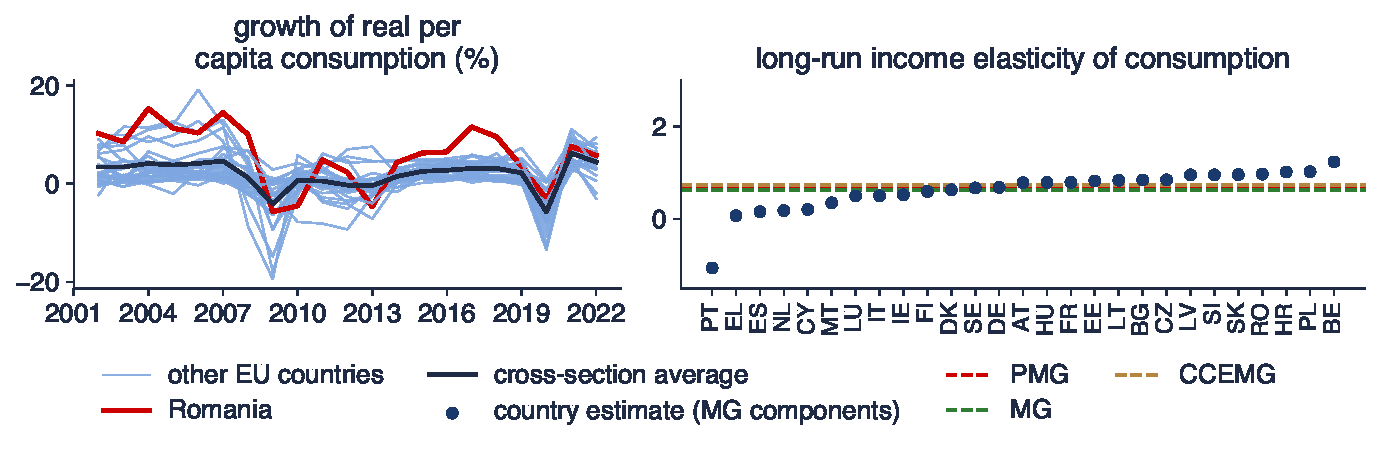
\includegraphics[width=0.97\textwidth,height=0.5\textheight,keepaspectratio]{ats_ch4_panel.pdf}
\end{center}
\vspace{-0.25cm}
\begin{itemize}
    \item Stînga: creșterea consumului (România cu roșu, media pe secțiune cu albastru închis); dreapta: elasticitățile de termen lung față de venit din ARDL-urile individuale, cu MG, PMG și CCEMG
    \item Elasticitățile pe țări variază între \ensuremath{-}1{,}06 și 1{,}23; România 0{,}97
\end{itemize}
\quantlet{ATS\_ch4\_panel}{\qlurl{ATS_ch4_panel}}
\end{frame}

\begin{frame}{Estimații de termen lung pentru UE-27}
\itemsize{\small}
\begin{center}
\footnotesize
\begin{tabular}{lccc}
\toprule
\textbf{Estimatorul} & $\theta_y$ & $\theta_\pi$ & $\phi$ \\
\midrule
MG & 0{,}63 (0{,}09) & 0{,}82 (0{,}32) & \ensuremath{-}0{,}43 (0{,}032) \\
PMG & 0{,}69 (0{,}04) & 0{,}41 (0{,}18) & \ensuremath{-}0{,}31 (0{,}028) \\
efecte fixe dinamice & 0{,}81 (0{,}03) & 0{,}01 (0{,}23) & \ensuremath{-}0{,}29 (0{,}025) \\
DOLS group mean & 0{,}77 (0{,}05) & \ensuremath{-}0{,}24 (0{,}17) & -- \\
CCEMG & 0{,}73 (0{,}05) & 0{,}10 (0{,}10) & -- \\
\bottomrule
\end{tabular}
\end{center}
\begin{itemize}
    \item Erorile standard în paranteze (MG, DOLS, CCEMG: dispersia estimațiilor pe țări; PMG: verosimilitatea; FE: grupate pe țări)
    \item Hausman MG față de PMG: $H = 2{,}41$, $\chi^2(2)$, $p = 0{,}300$; CD pentru reziduurile PMG: 30{,}9
\end{itemize}
\end{frame}

\begin{frame}{Interpretarea estimațiilor panel}
\itemsize{\small}
\begin{itemize}
    \item Elasticitatea față de venit se află între 0{,}63 (MG) și 0{,}81 (FE), clar sub unu: consumul nu urmează venitul unu la unu în 2001--2022
    \item Testul Hausman nu respinge coeficienții comuni, deci PMG este alegerea eficientă pentru efectul venitului
    \item Efectul inflației nu este robust: semnul și mărimea lui se schimbă cu estimatorul; nu raportați doar unul dintre ele
    \item Reziduurile PMG rămîn puternic dependente (CD = 30{,}9): erorile standard care ignoră șocurile comune sînt prea mici; CCEMG este reperul mai sigur
\end{itemize}
\end{frame}

\begin{frame}{VAR panel într-un slide}
\itemsize{\small}
\begin{itemize}
    \item $y_{it} = \mu_i + \sum_{j=1}^pA_jy_{i,t-j} + \varepsilon_{it}$: dinamică comună, efecte fixe pe țări \refHNR
    \item Pentru $T$ mic estimatorul within are o deplasare de ordinul $1/T$ (Nickell); estimăm prin GMM pe abateri ortogonale înainte, cu niveluri decalate ca instrumente \refAL
    \item Identificarea șocurilor ca în \atschlink{https://danpele.github.io/Advanced-Time-Series/RO/Cursuri/capitol3_modele_var_structurale_proiectii_locale.pdf}{Capitolul 3} (Cholesky, semne); răspunsurile la impuls și FEVD sînt comune tuturor țărilor
    \item Omogenitatea lui $A_j$ este ipoteza puternică: în panelurile macro cu $T$ moderat, VAR-urile mean group sau VAR-urile augmentate CCE sînt alternativele eterogene
\end{itemize}
\end{frame}

\begin{frame}{Recapitulare: serii de timp panel}
\itemsize{\small}
\begin{itemize}
    \item Testați întîi dependența între unități; dacă este puternică, folosiți CIPS și CCE, nu LLC/IPS și OLS comun
    \item Testele de cointegrare în panel diferă prin ipoteza nulă și prin restricția de factor comun; dezacordul este informativ
    \item MG pentru eterogenitate, PMG cînd teoria impune un termen lung comun, Hausman pentru decizie, CCE contra factorilor comuni
\end{itemize}
\end{frame}


%=============================================================================
\section{AI în descoperirea științifică}
%=============================================================================

\begin{frame}{O întrebare deschisă}
\itemsize{\small}
\begin{itemize}
    \item Este completă transmiterea pe termen lung a dobînzilor pieței monetare către dobînzile la credite în România și s-a schimbat după înăsprirea din 2022?
    \begin{itemize}
        \item formal: $H_0$: $\theta_{\text{credit}} = 1$ într-un VECM de rang 2 cu ROBOR slab exogen; față de o ruptură în $\theta$ sau în marjă în 2022
        \item infirmată de o respingere robustă: pentru numere de decalaje, cazuri deterministe și inferență bootstrap preînregistrate
    \end{itemize}
    \item Miza: viteza și completitudinea transmiterii decid cît trebuie să miște BNR dobînda de politică pentru a schimba condițiile de creditare
    \begin{itemize}
        \item literatura de pornire: \refdB, \refECR, \refJohD, \refCRT, \refPSSb
    \end{itemize}
\end{itemize}
\end{frame}

\begin{frame}{Bucla de cercetare cu un asistent AI}
\itemsize{\footnotesize}
\begin{itemize}
    \item Un asistent AI (un LLM precum Claude, ChatGPT, Gemini sau Copilot) accelerează fiecare etapă; Semantic Scholar și Elicit ajută la literatură
    \begin{itemize}
        \item \textbf{literatura}: \aiprompt{Listează studii recenzate despre transmiterea dobînzilor în Europa Centrală și de Est care folosesc VAR cointegrate sau ARDL; dă DOI-urile.} Apoi verificați fiecare DOI pe Crossref
        \item \textbf{ipoteza}: \aiprompt{Propune trei motive pentru care transmiterea către dobînzile la credite ar putea depăși unu și cîte o implicație testabilă pentru fiecare.}
        \item \textbf{cod și replicare}: cereți o funcție Johansen cu constantă restricționată, apoi reproduceți întîi o cifră cunoscută (valorile proprii din acest curs)
        \item \textbf{robustețe și critică}: \aiprompt{Joacă rolul unui recenzent ostil: enumeră toate alegerile de specificare care ar putea inversa testul transmiterii complete.}
    \end{itemize}
    \item Raportul: ce s-a cerut, ce s-a păstrat, ce s-a respins (AI\_USE.md, AI\_ERRORS.md)
\end{itemize}
\end{frame}

\begin{frame}{Verificări necesare}
\itemsize{\small}
\begin{itemize}
    \item Fiecare referință există și spune ce se afirmă (DOI-ul funcționează, titlul coincide, rezultatul se află în lucrare)
    \item Cazul determinist al valorilor critice corespunde modelului estimat (o eroare AI frecventă: valori ale cazului 3 pentru un model al cazului 2)
    \item Gradele de libertate ale fiecărui test LR asupra lui $\beta$ și $\alpha$ se numără de mînă
    \item Numărul de decalaje, cazul, eșantionul și tratarea perioadei 2008--2009 sînt fixate înaintea rezultatelor; toate variantele sînt raportate
    \item O afirmație de „transmitere completă” se verifică pe mulțimea de încredere a lui $\theta$, nu pe o singură valoare $p$
\end{itemize}
\end{frame}

\begin{frame}{Mini studiu de caz: estimația este robustă, verdictul nu}
\itemsize{\footnotesize}
\begin{center}
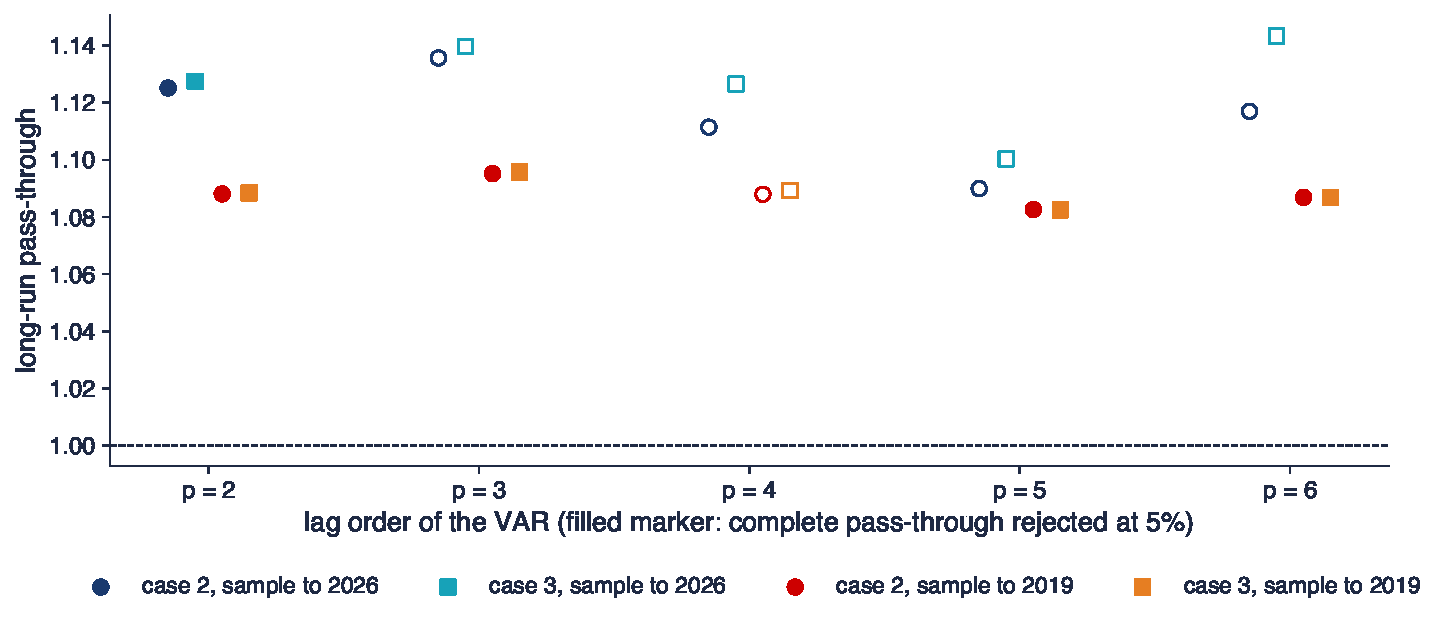
\includegraphics[width=0.97\textwidth,height=0.5\textheight,keepaspectratio]{ats_ch4_ai_case.pdf}
\end{center}
\vspace{-0.25cm}
\begin{itemize}
    \item Transmiterea pe termen lung către dobînda la credite în VECM de rang 2: decalaje $p = 2, \dots, 6$, cazurile 2 și 3, eșantioane care se încheie în 2019 și în 2026; marcaje pline: $\theta = 1$ respins la 5\%
    \item Toate cele 20 de estimații se află între 1{,}08 și 1{,}14, dar transmiterea completă este respinsă în 10 dintre ele: un rezumat AI care raportează o singură valoare $p$ „cu încredere” greșește
\end{itemize}
\quantlet{ATS\_ch4\_ai\_robustness}{\qlurl{ATS_ch4_ai_robustness}}
\end{frame}

\begin{frame}{Idee de proiect}
\itemsize{\small}
\begin{itemize}
    \item \textbf{Transmiterea dobînzilor în Europa Centrală și de Est}: întîi replicare, apoi extindere
    \begin{itemize}
        \item replicați: VECM-ul de rang 2 pentru România din acest curs (valorile proprii 0{,}244; 0{,}177; 0{,}017) și transmiterea ARDL 1{,}15
        \item extindeți: România, Ungaria, Cehia și Polonia; constante cu rupturi \refJMN\ în 2008 și 2022; teste de rang cu bootstrap wild; PMG între țări cu test Hausman; NARDL pentru transmitere asimetrică
        \item preînregistrați: variabilele, eșantionul, cazul, regula pentru decalaje, procedura pentru rang, restricțiile de testat și corecția pentru testare multiplă
    \end{itemize}
    \item Livrabilele urmează regulile cursului: repository, raport, AI\_USE.md, AI\_ERRORS.md, susținere orală
\end{itemize}
\end{frame}


%=============================================================================
\section{Încheiere}
%=============================================================================

\begin{frame}{Idei de reținut}
\itemsize{\small}
\begin{itemize}
    \item Johansen = regresie de rang redus; testul de rang este nestandard, depinde de caz și respinge prea des în eșantioane mici
    \item Pentru un rang dat, restricțiile asupra lui $\beta$ (economie) și $\alpha$ (exogenitate slabă) sînt teste $\chi^2$ obișnuite
    \item Cointegrarea furnizează zerouri de termen lung pentru analiza structurală: șocuri permanente și tranzitorii
    \item ARDL este un VECM condiționat: valabil sub exogenitate slabă și o singură relație, cu limite pentru eșantioane mici
    \item Panelurile adaugă putere, dar aduc eterogenitate și dependență între unități: întîi CD, apoi CIPS, MG/PMG și CCE
\end{itemize}
\end{frame}

\begin{frame}{Autoevaluare}
\itemsize{\small}
\begin{columns}[T]
\begin{column}{0.56\textwidth}
\begin{block}{Întrebări}
\begin{itemize}
    \item De ce dă o singură descompunere în valori proprii estimatorul ML al lui $\beta$ pentru orice rang?
    \item Ce caz determinist se potrivește pentru două dobînzi fără drift?
    \item Cîte grade de libertate are testul unui $\beta$ cunoscut cu $n_1 = 3$, $r = 2$?
    \item Ce vă permite exogenitatea slabă a lui ROBOR?
    \item De ce poate IPS să respingă o rădăcină unitară pe care CIPS nu o respinge?
\end{itemize}
\end{block}
\end{column}
\begin{column}{0.40\textwidth}
\begin{block}{Urmează: \atschlink{https://danpele.github.io/Advanced-Time-Series/RO/Cursuri/capitol5_bvar_modele_factoriale_nowcasting.pdf}{Capitolul 5}}
\begin{itemize}
    \item Modele VAR bayesiene, modele factoriale și nowcasting
    \item Shrinkage rezolvă problema numărului de parametri întîlnită în eșantioanele mici; factorii generalizează mediile pe secțiune din CCE
\end{itemize}
\end{block}
\end{column}
\end{columns}
\end{frame}


%=============================================================================
\section{Anexă}
%=============================================================================

\begin{frame}{Anexă: de la verosimilitate la valorile proprii}
\hypertarget{atsapp1}{}\atsappback{atssrc1}{Înapoi}
\itemsize{\small}
\begin{itemize}
    \item Pentru $\beta$ fixat: $|\hat\Omega(\beta)| = |S_{00} - S_{01}\beta(\beta'S_{11}\beta)^{-1}\beta'S_{10}|$; aplicăm determinantul partiționat matricei $\begin{pmatrix}S_{00} & S_{01}\beta\\ \beta'S_{10} & \beta'S_{11}\beta\end{pmatrix}$ în ambele ordini
    \item $|\hat\Omega(\beta)|\,|\beta'S_{11}\beta| = |S_{00}|\,|\beta'(S_{11} - S_{10}S_{00}^{-1}S_{01})\beta|$, de unde raportul de pe slide
    \item Scriem $\beta = S_{11}^{-1/2}\eta$: raportul devine $|\eta'(I - M)\eta|/|\eta'\eta|$ cu $M = S_{11}^{-1/2}S_{10}S_{00}^{-1}S_{01}S_{11}^{-1/2}$; minimul se obține cu vectorii proprii ai lui $M$ pentru cele mai mari $r$ valori proprii
    \item Minimul este $\prod_{i\le r}(1 - \lambda_i)$; rangurile imbricate au aceiași vectori proprii, deci statisticile LR sînt sume de termeni $-T\ln(1 - \hat\lambda_i)$
\end{itemize}
\end{frame}

\begin{frame}{Anexă: de ce $C = \beta_\perp(\alpha_\perp'\Gamma\beta_\perp)^{-1}\alpha_\perp'$}
\hypertarget{atsapp2}{}\atsappback{atssrc1}{Înapoi}
\itemsize{\small}
\begin{itemize}
    \item Înmulțim VECM cu $\alpha_\perp'$: $\alpha_\perp'\Delta y_t = \alpha_\perp'\sum_i\Gamma_i\Delta y_{t-i} + \alpha_\perp'\varepsilon_t$; prin însumare $\alpha_\perp'\Gamma y_t \approx \alpha_\perp'\sum_{s\le t}\varepsilon_s$ pînă la termeni staționari
    \item Descompunem $y_t = \beta(\beta'\beta)^{-1}\beta'y_t + \beta_\perp(\beta_\perp'\beta_\perp)^{-1}\beta_\perp'y_t$; prima parte este staționară
    \item Deci $\alpha_\perp'\Gamma\beta_\perp\,(\beta_\perp'\beta_\perp)^{-1}\beta_\perp'y_t \approx \alpha_\perp'\sum_s\varepsilon_s$; inversăm $\alpha_\perp'\Gamma\beta_\perp$ (condiția I(1)) și înmulțim la stînga cu $\beta_\perp$
    \item Rezultatul: partea nestaționară a lui $y_t$ este $\beta_\perp(\alpha_\perp'\Gamma\beta_\perp)^{-1}\alpha_\perp'\sum_s\varepsilon_s = C\sum_s\varepsilon_s$
\end{itemize}
\end{frame}

\begin{frame}{Anexă: verosimilitatea PMG}
\hypertarget{atsapp3}{}\atsappback{atssrc1}{Înapoi}
\itemsize{\small}
\begin{itemize}
    \item $\ell(\theta, \phi, \sigma^2) = -\sum_{i=1}^N\frac{T_i}{2}\ln(2\pi\sigma_i^2) - \sum_{i=1}^N\frac{1}{2\sigma_i^2}(\Delta y_i - \phi_i\xi_i(\theta))'H_i(\Delta y_i - \phi_i\xi_i(\theta))$
    \item $\xi_i(\theta) = y_{i,-1} - X_{i,-1}\theta$; $H_i$ elimină regresorii pe termen scurt și termenul liber ai țării
    \item Pentru $\theta$ dat, $\phi_i$ și $\sigma_i^2$ sînt OLS pe țări; verosimilitatea concentrată $-\sum_i\frac{T_i}{2}\ln\hat\sigma_i^2(\theta)$ se maximizează după $\theta$ (substituție înapoi sau Newton)
    \item $\hat\theta_{PMG}$ este consistent și asimptotic normal dacă $\phi_i < 0$ pentru orice $i$ și termenul lung este omogen; statutul I(0)/I(1) al lui $x$ nu contează, ca în ARDL
\end{itemize}
\end{frame}


%=============================================================================
\section{Bibliografie}
%=============================================================================

\begin{frame}{Bibliografie (1/5)}
\itemsize{\tiny}
\begin{itemize}
    \item Abrigo, M. R. M., \& Love, I. (2016). Estimation of panel vector autoregression in Stata. \textit{The Stata Journal}, 16(3), 778--804. \href{https://doi.org/10.1177/1536867X1601600314}{doi:10.1177/1536867X1601600314}
    \item Bacon, R. W. (1991). Rockets and feathers: The asymmetric speed of adjustment of UK retail gasoline prices to cost changes. \textit{Energy Economics}, 13(3), 211--218. \href{https://doi.org/10.1016/0140-9883(91)90022-R}{doi:10.1016/0140-9883(91)90022-R}
    \item Breitung, J., \& Pesaran, M. H. (2008). Unit roots and cointegration in panels. In L. Mátyás \& P. Sevestre (Eds.), \textit{The Econometrics of Panel Data} (pp.\ 279--322). Springer. \href{https://doi.org/10.1007/978-3-540-75892-1_9}{doi:10.1007/978-3-540-75892-1\_9}
    \item Cavaliere, G., Rahbek, A., \& Taylor, A. M. R. (2010). Cointegration rank testing under conditional heteroskedasticity. \textit{Econometric Theory}, 26(6), 1719--1760. \href{https://doi.org/10.1017/S0266466609990776}{doi:10.1017/S0266466609990776}
    \item Cavaliere, G., Rahbek, A., \& Taylor, A. M. R. (2012). Bootstrap determination of the co-integration rank in vector autoregressive models. \textit{Econometrica}, 80(4), 1721--1740. \href{https://doi.org/10.3982/ECTA9099}{doi:10.3982/ECTA9099}
    \item Chudik, A., \& Pesaran, M. H. (2015). Common correlated effects estimation of heterogeneous dynamic panel data models with weakly exogenous regressors. \textit{Journal of Econometrics}, 188(2), 393--420. \href{https://doi.org/10.1016/j.jeconom.2015.03.007}{doi:10.1016/j.jeconom.2015.03.007}
    \item de Bondt, G. J. (2005). Interest rate pass-through: Empirical results for the euro area. \textit{German Economic Review}, 6(1), 37--78. \href{https://doi.org/10.1111/j.1465-6485.2005.00121.x}{doi:10.1111/j.1465-6485.2005.00121.x}
    \item Égert, B., Crespo-Cuaresma, J., \& Reininger, T. (2007). Interest rate pass-through in Central and Eastern Europe: Reborn from ashes merely to pass away? \textit{Journal of Policy Modeling}, 29(2), 209--225. \href{https://doi.org/10.1016/j.jpolmod.2007.01.005}{doi:10.1016/j.jpolmod.2007.01.005}
    \item Engle, R. F., \& Granger, C. W. J. (1987). Co-integration and error correction: Representation, estimation, and testing. \textit{Econometrica}, 55(2), 251--276. \href{https://doi.org/10.2307/1913236}{doi:10.2307/1913236}
    \item Gonzalo, J., \& Ng, S. (2001). A systematic framework for analyzing the dynamic effects of permanent and transitory shocks. \textit{Journal of Economic Dynamics and Control}, 25(10), 1527--1546. \href{https://doi.org/10.1016/S0165-1889(99)00062-7}{doi:10.1016/S0165-1889(99)00062-7}
    \item Hamilton, J. D. (1994). \textit{Time Series Analysis}. Princeton University Press. \href{https://doi.org/10.2307/j.ctv14jx6sm}{doi:10.2307/j.ctv14jx6sm}
    \item Holtz-Eakin, D., Newey, W., \& Rosen, H. S. (1988). Estimating vector autoregressions with panel data. \textit{Econometrica}, 56(6), 1371--1395. \href{https://doi.org/10.2307/1913103}{doi:10.2307/1913103}
\end{itemize}
\end{frame}

\begin{frame}{Bibliografie (2/5)}
\itemsize{\tiny}
\begin{itemize}
    \item Im, K. S., Pesaran, M. H., \& Shin, Y. (2003). Testing for unit roots in heterogeneous panels. \textit{Journal of Econometrics}, 115(1), 53--74. \href{https://doi.org/10.1016/S0304-4076(03)00092-7}{doi:10.1016/S0304-4076(03)00092-7}
    \item Johansen, S. (1988). Statistical analysis of cointegration vectors. \textit{Journal of Economic Dynamics and Control}, 12(2--3), 231--254. \href{https://doi.org/10.1016/0165-1889(88)90041-3}{doi:10.1016/0165-1889(88)90041-3}
    \item Johansen, S. (1991). Estimation and hypothesis testing of cointegration vectors in Gaussian vector autoregressive models. \textit{Econometrica}, 59(6), 1551--1580. \href{https://doi.org/10.2307/2938278}{doi:10.2307/2938278}
    \item Johansen, S. (1992). Determination of cointegration rank in the presence of a linear trend. \textit{Oxford Bulletin of Economics and Statistics}, 54(3), 383--397. \href{https://doi.org/10.1111/j.1468-0084.1992.tb00008.x}{doi:10.1111/j.1468-0084.1992.tb00008.x}
    \item Johansen, S. (1995a). \textit{Likelihood-Based Inference in Cointegrated Vector Autoregressive Models}. Oxford University Press. \href{https://doi.org/10.1093/0198774508.001.0001}{doi:10.1093/0198774508.001.0001}
    \item Johansen, S. (1995b). Identifying restrictions of linear equations with applications to simultaneous equations and cointegration. \textit{Journal of Econometrics}, 69(1), 111--132. \href{https://doi.org/10.1016/0304-4076(94)01664-L}{doi:10.1016/0304-4076(94)01664-L}
    \item Johansen, S. (1995c). A statistical analysis of cointegration for I(2) variables. \textit{Econometric Theory}, 11(1), 25--59. \href{https://doi.org/10.1017/S0266466600009026}{doi:10.1017/S0266466600009026}
    \item Johansen, S. (2002). A small sample correction for the test of cointegrating rank in the vector autoregressive model. \textit{Econometrica}, 70(5), 1929--1961. \href{https://doi.org/10.1111/1468-0262.00358}{doi:10.1111/1468-0262.00358}
    \item Johansen, S., \& Juselius, K. (1990). Maximum likelihood estimation and inference on cointegration, with applications to the demand for money. \textit{Oxford Bulletin of Economics and Statistics}, 52(2), 169--210. \href{https://doi.org/10.1111/j.1468-0084.1990.mp52002003.x}{doi:10.1111/j.1468-0084.1990.mp52002003.x}
    \item Johansen, S., Mosconi, R., \& Nielsen, B. (2000). Cointegration analysis in the presence of structural breaks in the deterministic trend. \textit{The Econometrics Journal}, 3(2), 216--249. \href{https://doi.org/10.1111/1368-423X.00047}{doi:10.1111/1368-423X.00047}
    \item Juselius, K. (2006). \textit{The Cointegrated VAR Model: Methodology and Applications}. Oxford University Press. \href{https://doi.org/10.1093/oso/9780199285662.001.0001}{doi:10.1093/oso/9780199285662.001.0001}
    \item Kao, C. (1999). Spurious regression and residual-based tests for cointegration in panel data. \textit{Journal of Econometrics}, 90(1), 1--44. \href{https://doi.org/10.1016/S0304-4076(98)00023-2}{doi:10.1016/S0304-4076(98)00023-2}
\end{itemize}
\end{frame}

\begin{frame}{Bibliografie (3/5)}
\itemsize{\tiny}
\begin{itemize}
    \item Kapetanios, G., Pesaran, M. H., \& Yamagata, T. (2011). Panels with non-stationary multifactor error structures. \textit{Journal of Econometrics}, 160(2), 326--348. \href{https://doi.org/10.1016/j.jeconom.2010.10.001}{doi:10.1016/j.jeconom.2010.10.001}
    \item Kilian, L., \& Lütkepohl, H. (2017). \textit{Structural Vector Autoregressive Analysis}. Cambridge University Press. \href{https://doi.org/10.1017/9781108164818}{doi:10.1017/9781108164818}
    \item King, R. G., Plosser, C. I., Stock, J. H., \& Watson, M. W. (1991). Stochastic trends and economic fluctuations. \textit{American Economic Review}, 81(4), 819--840. \href{https://www.jstor.org/stable/2006644}{jstor.org}
    \item Kripfganz, S., \& Schneider, D. C. (2020). Response surface regressions for critical value bounds and approximate p-values in equilibrium correction models. \textit{Oxford Bulletin of Economics and Statistics}, 82(6), 1456--1481. \href{https://doi.org/10.1111/obes.12377}{doi:10.1111/obes.12377}
    \item Levin, A., Lin, C.-F., \& Chu, C.-S. J. (2002). Unit root tests in panel data: Asymptotic and finite-sample properties. \textit{Journal of Econometrics}, 108(1), 1--24. \href{https://doi.org/10.1016/S0304-4076(01)00098-7}{doi:10.1016/S0304-4076(01)00098-7}
    \item Lütkepohl, H. (2005). \textit{New Introduction to Multiple Time Series Analysis}. Springer. \href{https://doi.org/10.1007/978-3-540-27752-1}{doi:10.1007/978-3-540-27752-1}
    \item MacKinnon, J. G., Haug, A. A., \& Michelis, L. (1999). Numerical distribution functions of likelihood ratio tests for cointegration. \textit{Journal of Applied Econometrics}, 14(5), 563--577. \href{https://doi.org/10.1002/(SICI)1099-1255(199909/10)14:5\%3C563::AID-JAE530\%3E3.0.CO\%3B2-R}{doi:10.1002/(SICI)1099-1255(199909/10)14:5\textless{}563::AID-JAE530\textgreater{}3.0.CO;2-R}
    \item Narayan, P. K. (2005). The saving and investment nexus for China: Evidence from cointegration tests. \textit{Applied Economics}, 37(17), 1979--1990. \href{https://doi.org/10.1080/00036840500278103}{doi:10.1080/00036840500278103}
    \item Nickell, S. (1981). Biases in dynamic models with fixed effects. \textit{Econometrica}, 49(6), 1417--1426. \href{https://doi.org/10.2307/1911408}{doi:10.2307/1911408}
    \item Osterwald-Lenum, M. (1992). A note with quantiles of the asymptotic distribution of the maximum likelihood cointegration rank test statistics. \textit{Oxford Bulletin of Economics and Statistics}, 54(3), 461--472. \href{https://doi.org/10.1111/j.1468-0084.1992.tb00013.x}{doi:10.1111/j.1468-0084.1992.tb00013.x}
    \item Pantula, S. G. (1989). Testing for unit roots in time series data. \textit{Econometric Theory}, 5(2), 256--271. \href{https://doi.org/10.1017/S0266466600012421}{doi:10.1017/S0266466600012421}
    \item Pedroni, P. (1999). Critical values for cointegration tests in heterogeneous panels with multiple regressors. \textit{Oxford Bulletin of Economics and Statistics}, 61(S1), 653--670. \href{https://doi.org/10.1111/1468-0084.0610s1653}{doi:10.1111/1468-0084.0610s1653}
\end{itemize}
\end{frame}

\begin{frame}{Bibliografie (4/5)}
\itemsize{\tiny}
\begin{itemize}
    \item Pedroni, P. (2001). Purchasing power parity tests in cointegrated panels. \textit{The Review of Economics and Statistics}, 83(4), 727--731. \href{https://doi.org/10.1162/003465301753237803}{doi:10.1162/003465301753237803}
    \item Pedroni, P. (2004). Panel cointegration: Asymptotic and finite sample properties of pooled time series tests with an application to the PPP hypothesis. \textit{Econometric Theory}, 20(3), 597--625. \href{https://doi.org/10.1017/S0266466604203073}{doi:10.1017/S0266466604203073}
    \item Pesaran, M. H. (2006). Estimation and inference in large heterogeneous panels with a multifactor error structure. \textit{Econometrica}, 74(4), 967--1012. \href{https://doi.org/10.1111/j.1468-0262.2006.00692.x}{doi:10.1111/j.1468-0262.2006.00692.x}
    \item Pesaran, M. H. (2007). A simple panel unit root test in the presence of cross-section dependence. \textit{Journal of Applied Econometrics}, 22(2), 265--312. \href{https://doi.org/10.1002/jae.951}{doi:10.1002/jae.951}
    \item Pesaran, M. H. (2015a). Testing weak cross-sectional dependence in large panels. \textit{Econometric Reviews}, 34(6--10), 1089--1117. \href{https://doi.org/10.1080/07474938.2014.956623}{doi:10.1080/07474938.2014.956623}
    \item Pesaran, M. H. (2015b). \textit{Time Series and Panel Data Econometrics}. Oxford University Press. \href{https://doi.org/10.1093/acprof:oso/9780198736912.001.0001}{doi:10.1093/acprof:oso/9780198736912.001.0001}
    \item Pesaran, M. H. (2021). General diagnostic tests for cross-sectional dependence in panels. \textit{Empirical Economics}, 60(1), 13--50. \href{https://doi.org/10.1007/s00181-020-01875-7}{doi:10.1007/s00181-020-01875-7}
    \item Pesaran, M. H., \& Shin, Y. (1998). An autoregressive distributed-lag modelling approach to cointegration analysis. In S. Strøm (Ed.), \textit{Econometrics and Economic Theory in the 20th Century: The Ragnar Frisch Centennial Symposium} (pp.\ 371--413). Cambridge University Press. \href{https://doi.org/10.1017/CCOL0521633230.011}{doi:10.1017/CCOL0521633230.011}
    \item Pesaran, M. H., Shin, Y., \& Smith, R. J. (2001). Bounds testing approaches to the analysis of level relationships. \textit{Journal of Applied Econometrics}, 16(3), 289--326. \href{https://doi.org/10.1002/jae.616}{doi:10.1002/jae.616}
    \item Pesaran, M. H., Shin, Y., \& Smith, R. P. (1999). Pooled mean group estimation of dynamic heterogeneous panels. \textit{Journal of the American Statistical Association}, 94(446), 621--634. \href{https://doi.org/10.1080/01621459.1999.10474156}{doi:10.1080/01621459.1999.10474156}
    \item Pesaran, M. H., \& Smith, R. (1995). Estimating long-run relationships from dynamic heterogeneous panels. \textit{Journal of Econometrics}, 68(1), 79--113. \href{https://doi.org/10.1016/0304-4076(94)01644-F}{doi:10.1016/0304-4076(94)01644-F}
    \item Phillips, P. C. B., \& Hansen, B. E. (1990). Statistical inference in instrumental variables regression with I(1) processes. \textit{The Review of Economic Studies}, 57(1), 99--125. \href{https://doi.org/10.2307/2297545}{doi:10.2307/2297545}
\end{itemize}
\end{frame}

\begin{frame}{Bibliografie (5/5)}
\itemsize{\tiny}
\begin{itemize}
    \item Phillips, P. C. B., \& Moon, H. R. (1999). Linear regression limit theory for nonstationary panel data. \textit{Econometrica}, 67(5), 1057--1111. \href{https://doi.org/10.1111/1468-0262.00070}{doi:10.1111/1468-0262.00070}
    \item Reinsel, G. C., \& Ahn, S. K. (1992). Vector autoregressive models with unit roots and reduced rank structure: Estimation, likelihood ratio test, and forecasting. \textit{Journal of Time Series Analysis}, 13(4), 353--375. \href{https://doi.org/10.1111/j.1467-9892.1992.tb00113.x}{doi:10.1111/j.1467-9892.1992.tb00113.x}
    \item Saikkonen, P. (1991). Asymptotically efficient estimation of cointegration regressions. \textit{Econometric Theory}, 7(1), 1--21. \href{https://doi.org/10.1017/S0266466600004217}{doi:10.1017/S0266466600004217}
    \item Shin, Y., Yu, B., \& Greenwood-Nimmo, M. (2014). Modelling asymmetric cointegration and dynamic multipliers in a nonlinear ARDL framework. In R. C. Sickles \& W. C. Horrace (Eds.), \textit{Festschrift in Honor of Peter Schmidt} (pp.\ 281--314). Springer. \href{https://doi.org/10.1007/978-1-4899-8008-3_9}{doi:10.1007/978-1-4899-8008-3\_9}
    \item Stock, J. H., \& Watson, M. W. (1993). A simple estimator of cointegrating vectors in higher order integrated systems. \textit{Econometrica}, 61(4), 783--820. \href{https://doi.org/10.2307/2951763}{doi:10.2307/2951763}
    \item Swensen, A. R. (2006). Bootstrap algorithms for testing and determining the cointegration rank in VAR models. \textit{Econometrica}, 74(6), 1699--1714. \href{https://doi.org/10.1111/j.1468-0262.2006.00723.x}{doi:10.1111/j.1468-0262.2006.00723.x}
    \item Toda, H. Y., \& Yamamoto, T. (1995). Statistical inference in vector autoregressions with possibly integrated processes. \textit{Journal of Econometrics}, 66(1--2), 225--250. \href{https://doi.org/10.1016/0304-4076(94)01616-8}{doi:10.1016/0304-4076(94)01616-8}
    \item Westerlund, J. (2007). Testing for error correction in panel data. \textit{Oxford Bulletin of Economics and Statistics}, 69(6), 709--748. \href{https://doi.org/10.1111/j.1468-0084.2007.00477.x}{doi:10.1111/j.1468-0084.2007.00477.x}
\end{itemize}
\end{frame}

\end{document}
